% Options for packages loaded elsewhere
\PassOptionsToPackage{unicode}{hyperref}
\PassOptionsToPackage{hyphens}{url}
\documentclass[
]{article}
\usepackage{xcolor}
\usepackage{amsmath,amssymb}
\setcounter{secnumdepth}{-\maxdimen} % remove section numbering
\usepackage{iftex}
\ifPDFTeX
  \usepackage[T1]{fontenc}
  \usepackage[utf8]{inputenc}
  \usepackage{textcomp} % provide euro and other symbols
\else % if luatex or xetex
  \usepackage{unicode-math} % this also loads fontspec
  \defaultfontfeatures{Scale=MatchLowercase}
  \defaultfontfeatures[\rmfamily]{Ligatures=TeX,Scale=1}
\fi
\usepackage{lmodern}
\ifPDFTeX\else
  % xetex/luatex font selection
\fi
% Use upquote if available, for straight quotes in verbatim environments
\IfFileExists{upquote.sty}{\usepackage{upquote}}{}
\IfFileExists{microtype.sty}{% use microtype if available
  \usepackage[]{microtype}
  \UseMicrotypeSet[protrusion]{basicmath} % disable protrusion for tt fonts
}{}
\makeatletter
\@ifundefined{KOMAClassName}{% if non-KOMA class
  \IfFileExists{parskip.sty}{%
    \usepackage{parskip}
  }{% else
    \setlength{\parindent}{0pt}
    \setlength{\parskip}{6pt plus 2pt minus 1pt}}
}{% if KOMA class
  \KOMAoptions{parskip=half}}
\makeatother
\usepackage{longtable,booktabs,array}
\usepackage{caption}
\captionsetup[table]{skip=6pt}
\newcounter{none} % for unnumbered tables
\usepackage{calc} % for calculating minipage widths
% Correct order of tables after \paragraph or \subparagraph
\usepackage{etoolbox}
\makeatletter
\patchcmd\longtable{\par}{\if@noskipsec\mbox{}\fi\par}{}{}
\makeatother
\usepackage{graphicx}
\makeatletter
\newsavebox\pandoc@box
\newcommand*\pandocbounded[1]{% scales image to fit in text height/width
  \sbox\pandoc@box{#1}%
  \Gscale@div\@tempa{\textheight}{\dimexpr\ht\pandoc@box+\dp\pandoc@box\relax}%
  \Gscale@div\@tempb{\linewidth}{\wd\pandoc@box}%
  \ifdim\@tempb\p@<\@tempa\p@\let\@tempa\@tempb\fi% select the smaller of both
  \ifdim\@tempa\p@<\p@\scalebox{\@tempa}{\usebox\pandoc@box}%
  \else\usebox{\pandoc@box}%
  \fi%
}
% Set default figure placement to htbp
\def\fps@figure{htbp}
\makeatother
\setlength{\emergencystretch}{3em} % prevent overfull lines
\providecommand{\tightlist}{%
  \setlength{\itemsep}{0pt}\setlength{\parskip}{0pt}}
\usepackage{bookmark}
\IfFileExists{xurl.sty}{\usepackage{xurl}}{} % add URL line breaks if available
\urlstyle{same}
% fallback for those not using the hyperref driver hyperxmp:
\makeatletter
\@ifundefined{xmpquote}{\newcommand{\xmpquote}[1]{#1}}{}
\makeatother
\hypersetup{
  pdftitle={A Climate Zone-Informed Parameter Evolution Framework (CZIPEF) for Assessing Catchment Vulnerability to Climate Change Under Model Parameter Non-Stationarity},
  hidelinks,
  pdfcreator={LaTeX via pandoc}}

\title{A Climate Zone-Informed Parameter Evolution Framework (CZIPEF)
for Assessing Catchment Vulnerability to Climate Change Under Model
Parameter Non-Stationarity}
\author{}
\date{}

\begin{document}
\maketitle

Ankit Deshmukh\textsuperscript{1}*, Shreekant
Varshney\textsuperscript{2}

\textsuperscript{1}Department of Civil Engineering, School of
Technology, Pandit Deendayal Energy University, Gandhinagar, 382426,
India

\textsuperscript{2}Department of Mathematics, School of Technology,
Pandit Deendayal Energy University, Gandhinagar, 382426, India

*Correspondence: Ankit Deshmukh (deshmukh.acad@gmail.com)

\section{Abstract}\label{abstract}

Climate change significantly impacts standard hydrological modeling
paradigms by invalidating the core assumption of parameter stationarity,
hence generating critical uncertainties in catchment management and
hydrological projections. Traditional calibration strategies treat model
parameters as temporally invariant, considering their long-term validity
for streamflow predictions; however, evolving climatic conditions and
subtle catchment modifications systematically undermine this assumption,
resulting in significant inconsistencies in our understanding of
hydrological vulnerability. The present investigation addresses these
limitations through an in-depth assessment of parameter non-stationarity
within the Hydrologiska Byråns Vattenbalansavdelning (HBV) model,
employing a bottom-up exploratory framework that explicitly investigates
hydrological projection sensitivity to parameter shifts across diverse
climate scenarios. Our methodology integrates Köppen-Geiger climatic
classifications with non-stationary parameter dynamics, producing a
novel vulnerability assessment framework that~quantifies catchment
susceptibility through climatic inputs threshold-based approaches. The
analysis shows that the framework changes the estimated vulnerability of
most catchments but not in a consistent direction. Of 332 candidate
catchments, 222 pass the calibration and climate-zone requirements and
form the analysed sample. For mean annual runoff, the climate
zone-informed framework changes the precipitation threshold in 72\% of
these catchments (38\% higher and 34\% lower than the stationary
framework, 28\% identical), but the median difference is zero and the
two thresholds agree only weakly (slope 0.31, R2 = 0.14). The
temperature threshold is identifiable in fewer than 7\% of catchments,
and the supplementary low-flow and high-flow indicators give
identifiable precipitation thresholds in only 10-26\% of catchments, so
the primary conclusions rest on mean annual runoff. These findings
highlight the inadequate performance of the existing methodologies in
capturing long-term hydrological uncertainty and highlight the crucial
demand for a major paradigm shift from stationarity-based
simplifications toward complex, climate- and biome-informed modeling
approaches. Such techniques must rigorously analyze parameter
sensitivity and environmental thresholds under anticipated climate
change scenarios, ultimately enabling more robust and appropriate
hydrological estimates for sustainable catchment management.

\textbf{Keywords:} Parameter non-stationarity, Climate zones, Streamflow
indices, Climate

change, Hydrological modelling, HBV, Köppen-Geiger.

\section{1. Introduction}\label{introduction}

The identification of catchment vulnerability to climate change
indicates an essential concern in contemporary water resource
management, particularly as water resources serve as the primary
societal driver amid accelerating climate change trends observed over
the past decade (Markovic et al., 2017; Parmesan et al., 2022). The
inherent uncertainty associated with greenhouse gas emission projections
introduces substantial complexity into global-scale climatic driver
forecasting, thereby compromising the reliability of long-term climate
assessments (Calvin et al., 2023; den Elzen et al., 2025). Specifically,
uncertainties from CO\textsubscript{2} concentration scenarios propagate
across the modeling chain, resulting in reduced accuracy of long-term
precipitation and temperature estimates (den Elzen et al., 2025; Qasmi
\& Ribes, 2022). At the catchment scale, precise precipitation and
temperature flux estimates are necessary requirements for reliable
runoff simulation utilizing selected hydrological models (Ajjur \&
Al-Ghamdi, 2024; Melo et al., 2024; Wu et al., 2021). Although numerous
hydrological models are available that utilize climatic inputs in
conjunction with calibrated parameters to simulate runoff processes, the
inherent uncertainty in input climate projections, compounded by model
parameter uncertainty, generates substantial noise in runoff projections
that may significantly deviate from actual catchment flows
(Kunnath-Poovakka et al., 2021; Teweldebrhan et al., 2018; Wu et al.,
2021). Consequently, when catchment vulnerability indicators are derived
from such uncertain simulated runoff data, including metrics related to
annual water availability, low flow conditions, or flood events, the
resulting assessments may be significantly impacted (Borzı̀, 2023; Forte
et al., 2025; Song et al., 2022). Therefore, as uncertainty accumulates
through each successive modeling step, the computed vulnerability
thresholds may become statistically insignificant and potentially
incorrectly represent actual catchment conditions, thereby affecting the
reliability of climate change adaptation strategies (Rodrı́guez-Rincón et
al., 2015; Xia et al., 2023).

The top-down approach, additionally referred to as the first
generation~or~impacts framework,~provides a climate-driven methodology
that begins with global climate forecasts and systematically downscales
them to analyze local-scale impacts (Eicken et al., 2021; Kucharski et
al., 2024). This technique primarily follows a linear causality chain:
emissions scenarios followed by climate models, then model simulations,
and lastly the vulnerability assessment (Eicken et al., 2021; van
Werkhoven et al., 2008) . Top-down assessments are characterized by
their emphasis on globally consistent frameworks that reflect
macroeconomic and market feedback (Girard et al., 2015; Lemoine \&
Kapnick, 2016). The methodology commonly incorporates General
Circulation Models (GCMs) and Regional Climate Models (RCMs) to forecast
future climatic variables, which are subsequently combined with sectoral
models (hydrological, agricultural, or ecological) to simulate
biophysical responses (Carter et al., 1998). Using the up-to-date
understanding of climate-system interactions, top-down techniques
provide reliable assessments that effectively depict the direct
cause-and-effect relationships between climate stimuli and biophysical
consequences (Conway et al., 2019; Girard et al., 2015). They are
particularly suitable for forecasting large-scale climate change
implications and may forecast system states further into the future
through integrated modeling frameworks (Conway et al., 2019). These
approaches are most effective for national-level assessments and
strategic planning situations where broad-scale patterns and trends are
more significant than local specificities (Nair \& Bharat, 2011). They
provide standardized procedures that enable cross-regional comparisons
and facilitate policy creation at macro dimensions but may not be
sufficiently effective for regional or catchment-scale under increasing
uncertainty in the various stages in the vulnerability assessment.

Another modeling paradigm is bottom-up approach that instead of
predicting future climate impacts, focus on identifying what makes
people and systems vulnerable. They are derived from catastrophe risk
reduction, emergency aid, and community development traditions (Conway
et al., 2019; Girard et al., 2015). This model prioritizes the
development context and underlying causes of vulnerability, specifically
recognizing that different social groups demonstrate variable
vulnerability to climate change impacts (Thomas et al., 2019). These
bottom-up assessments are fundamentally participative and conducted at
local levels (households, communities, or individual catchments)
(Maharjan et al., 2017). They primarily focus on identifying present
vulnerability rather than forecasting future conditions, while
participatory scenario planning approaches are increasingly incorporated
(Petzold et al., 2024).

The fundamental strength of bottom-up techniques exists in their
capacity to identify specific vulnerable groups and demonstrate
differential vulnerabilities across social strata (Conway et al., 2019;
Eicken et al., 2021). Their participatory aspect makes them extremely
beneficial for involving multiple stakeholders and enabling community
voices in adaptation planning (Sartorius et al., 2024; Wamsler,
2017).These assessments are effective at small spatial scales where
large-scale simulation models cannot deliver credible insights.
Bottom-up approaches are particularly helpful for local adaptation
initiatives and community-based natural resource management. They
provide an in-depth understanding of local strategies for coping,
resource constraints, and institutional capacities that influence
adaptive responses. The fundamental drawback of top-down techniques is
in their limited capacity to capture sectoral details and the complexity
of local demand-supply dynamics (Nair \& Bharat, 2011). By adopting
globally scaled models, they often lack precision for regional-scale
assessments and may insufficiently capture the social components of
socio-ecological systems (Girard et al., 2015).

Moreover, recent developments include the establishment of exploratory
modeling frameworks that address fundamental uncertainties associated
with climate change assessment(Brown, 2011; Haasnoot et al., 2013).
These techniques, demonstrated in (Deshmukh \& Singh, 2016) study,
involve decision-scaling methodologies that begin with
stakeholder-defined vulnerability thresholds rather than climate
projections (Deshmukh \& Singh, 2016). The exploratory methodology
measures catchment vulnerability through systematic stress-testing
across a broad spectrum of probable climate conditions, identifying
essential thresholds over which systems become vulnerable regardless of
specific future scenarios (Deshmukh \& Singh, 2016, 2019). This
methodology incorporates features of both top-down (via systematic
scenario exploration) and bottom-up (through stakeholder-defined
criteria) methodologies.

The fundamental concept of stationarity, predicated on the assumption
that ecosystems in nature fluctuate within an invariant envelope of
variability, has traditionally served as the foundation for hydrological
modeling and water resources planning frameworks (Arnell, 1999; Milly et
al., 2008). Under this standard paradigm, model parameters are validated
using historical data and subsequently assumed to be temporally
invariant throughout future projection periods. Nevertheless,
accumulating scientific evidence progressively reveals that hydrological
systems are exhibiting pronounced non-stationary behavior, mainly due to
global climate change and substantial environmental alterations (Razavi
et al., 2015). Consequently, these systemic changes fundamentally affect
the reliability of traditional calibration methodologies and reduce
model predictive capabilities, thereby necessitating the development of
adaptive modeling frameworks that enable parameter evolution in response
to dynamic climatic and environmental conditions (Agilan \& Umamahesh,
2017).

Recent large-scale analytical investigations have extensively
established the widespread presence and inherent complexity of parameter
non-stationarity across varied hydrological systems. For instance,
comprehensive sensitivity analyses conducted across 605 U.S. basins
demonstrated a systematic decrease in the influence of snow-melt
parameters, concomitant with an increasing sensitivity of soil- and
evapotranspiration-related parameters under RCP8.5 warming scenarios,
with approximately 55\% of catchments experiencing fundamental
reorganization of their dominant hydrological controls (Melsen \& Guse,
2021a). Similarly, analogous observations have emerged from
investigations across European and Indian subcontinent watersheds, where
previously robust hydrological models have required substantial
adaptation to accommodate shifting precipitation extremes and
anthropogenic water withdrawals to maintain acceptable performance
levels (Chuphal \& Mishra, 2023; W. Zhang et al., 2024). The complexity
of parameter drift becomes particularly apparent within the context of
water shortage monitoring and drought forecasting applications, as model
inefficiency may directly prevent effective adaptation strategies and
resource management planning initiatives. Specifically, Bayesian
hierarchical modeling methods have conclusively demonstrated that
excluding non-stationarity systematically minimizes drought
severity-duration-frequency relationships, while incorporating dynamic
parameter evolution significantly decreases projection uncertainty and
enhances predictive reliability (Salakpi et al., 2022; Samantaray et
al., 2025). Experimental findings~derived from split-sample and
sliding-window analytical approaches further demonstrate that optimal
parameter values can exhibit significant fluctuations within decadal
timeframes, thereby violating fundamental ergodic assumptions and
challenging conventional model calibration methodologies (Lan et al.,
2020; X. Zhang \& Liu, 2021).

Non-stationarity typically emerges when fundamental statistical
properties, governing critical processes such as snow accumulation
dynamics, soil moisture retention mechanisms, and evapotranspiration
rates, deviate beyond their historical estimation ranges, frequently as
a consequence of evolving precipitation regimes, systematic temperature
shifts, and land-cover transformations (Pathiraja et al., 2018). In the
context of regional-scale modelling attempts, parameter adaptability
demonstrates complex dependencies on the features of the prevalent
climate regime. Climate-induced transitions across established boundary
classifications, such as those indicated by the Köppen--Geiger climate
classification system, might effectively render existing parameter
transfer functions irrelevant and decrease model applicability (Melsen
\& Guse, 2021a).

The Köppen--Geiger climate classification (Köppen \& Geiger, 1930)
system is among the most widely utilized frameworks in climate,
hydrological, and ecological research. It offers a systematic basis for
characterizing global temperature--precipitation regimes while providing
standardized criteria for the delineation of distinct hydroclimatic
zones (Peel et al., 2007). Deshmukh \& Singh (2019) also, proposed a
Whittaker biome‐based framework to compute catchment vulnerabilities.
Recent methodological developments have enabled high-resolution
extensions of this categorization system, which now permit precise
projection of climate zone boundaries up to 2099, hence facilitating
detailed tracking of hydroclimatic alterations at fine spatial scales
(Beck et al., 2023). Consequently, the integration of both contemporary
and projected Köppen--Geiger classifications as temporally evolving
components within hydrological modeling frameworks presents substantial
potential for controlling and physically contextualizing parameter drift
patterns under anticipated future climate conditions. Recent empirical
investigations suggest that patterns of parameter non-stationarity
exhibit marked variability across distinct climate zones. Studies
indicate that arid regions demonstrate increased sensitivity in soil
moisture and catchment parameters (Mupepi et al., 2025), while temperate
and continental regions display increasing non-stationarity in snow and
evapotranspiration-related parameters under progressive warming
scenarios (Vormoor et al., 2021; Son \& Tague, 2019). This study
compares two modeling approaches: a Stationary Parameter Framework
(SPF), which assumes temporally invariant hydrological parameters under
climate change, and the proposed Climate Zone-Informed Parameter
Evolution Framework (CZIPEF), which explicitly integrates evolving
Köppen--Geiger climate zones to model parameter adaptation under
non-stationary climatic conditions. In this study the Beck et al. (2023)
scheme supplies the class definitions and the delta-change logic: the
observed 1981--2010 monthly climatology is perturbed and reclassified,
so the resulting maps are a controlled delta-change experiment rather
than a CMIP6 projection or a pixel-level comparison with the Beck et al.
rasters.

Despite the wide range of research that has independently investigated
parameter drift phenomena and the application of climate classifications
for regionalization purposes, a significant methodological gap persists
such as no comprehensive framework has explicitly established the
linkage between parameter non-stationarity and Köppen--Geiger climate
zone transitions under future climate scenarios. This crucial
relationship is essential for characterizing the temporal and spatial
parameters under which model reconfiguration becomes necessary as
hydrological basins migrate toward drier or warmer climatic
classifications. Therefore, the present investigation addresses such a
critical research gap by systematically evaluating whether hydrological
model parameters require structured adjustment as catchments evolve
Köppen--Geiger classification transitions from the historical period to
the to the projected climate scenarios.

Despite substantial methodological advances in recent years, significant
challenges persist in establishing the fundamental physical factors
underlying parameter non-stationarity, comprehensively understanding how
it appears across multiple spatial and temporal scales, and developing
computationally efficient, process-informed calibration strategies that
maintain theoretical reliability. Addressing these important knowledge
gaps is essential for improving adaptive hydrological modeling paradigms
and establishing robust water resources management frameworks capable of
systematically accounting for parameter uncertainty in the context of
accelerated anthropogenic climate change.

\emph{The primary objective of this investigation is to advance a
comprehensive catchment vulnerability assessment framework that
explicitly incorporates model non-stationarity considerations, with
particular emphasis on integrating Köppen--Geiger climate
classifications as a fundamental structuring principle.} While the
majority of existing vulnerability assessment frameworks depend
primarily on raw climatic variables such as temperature and
precipitation, they frequently neglect the critical ecological
thresholds and hydro-climatological regime characteristics embedded
within the Köppen--Geiger classification system (Lukasiewicz et al.,
2013). This study proposes a novel methodological approach for
quantifying catchment vulnerability to climate change through the
strategic utilization of the Köppen--Geiger classification system,
explicitly recognizing that climate zones are projected to experience
substantial spatial reconfiguration under future climate scenarios (Beck
et al., 2018; Song et al., 2025). To systematically address this
essential knowledge gap, the framework described herein attempts to
analyze vulnerability change thresholds that directly influence the
assessment of parameter non-stationarity in hydrological modeling
applications.

Moreover, whereas parameter sensitivity has been demonstrated to vary
significantly across distinct environmental regimes (Demaria et al.,
2007; Melsen \& Guse, 2021b; van Werkhoven et al., 2008) no prior
studies have thoroughly evaluated how such non-stationarity emerges over
the complete spectrum of Köppen--Geiger climate classifications.
Similarly, although non-stationary biases in climate model outputs are
well-documented in the literature (Khan et al., 2020), their systematic
propagation through the Köppen--Geiger classification system into
time-varying vulnerability assessments has yet to be comprehensively
quantified or characterized. Additionally, the primary emphasis of
current vulnerability frameworks on comprehensive, temperate catchment
systems (Avanzi et al., 2020) renders monsoonal and semi-arid climate
zones, particularly relevant for South Asian regional applications,
significantly neglected in the existing scientific literature.

Within this broader research context, the primary objective of this
investigation is to construct and implement an integrated
non-stationary, Köppen-informed vulnerability assessment paradigm that
systematically addresses these previously overlooked methodological
features. By explicitly establishing relationships between climate zone
transitions, hydrological parameter dynamics, and vulnerability
threshold identification, this framework aims not only to advance
fundamental methodological accuracy~within the area of research but also
to provide a robust foundation for translating complex non-stationary
hydrological processes into feasible, science-based adaptation
strategies at the catchment scale (Bouaziz et al., 2022; Kumar et al.,
2023).

The organization of the study is structured as follows: Section 1
provides an introduction and identifying existing research gaps,
particularly concerning approaches addressing parameter
non-stationarity. In Section 2, the study area and the datasets utilized
are described. The catchment vulnerability estimation methodology
framework, including a detailed description of the models implemented,
is laid out in Section 3. The Results section 4 includes vulnerability
threshold identification along with other essential parameters
integrated into the final model implementation. Subsequently, section 5
interprets the analysis, specifically exploring the spatial patterns of
vulnerabilities and measuring the influence of both stationary and
non-stationary parameter circumstances on vulnerability thresholds.
Finally, Section 6 synthesizes the study, provides an overall
perspective, and poses open-ended questions for
highlighting~advancements and future research directions.

\section{2. Study Area and Data}\label{study-area-and-data}

The proposed~investigation utilizes the catchment attributes and
meteorology for the large-sample (CAMELS) dataset (Addor et al., 2017)
and includes 671 minimally transformed catchments throughout the
continental United States. The catchments have been selected from the
USGS hydro-climatic data network to minimize anthropogenic influence and
maximize natural variability for hydrological modeling and analysis. The
dataset covers numerous catchment attributes such as topographical,
climatic, soil properties, land cover, vegetation, and geological,
together with hydro-climatic time-series. The daily time-series data
from CAMELS-USA comprises precipitation, streamflow, discharge, maximum
temperature, and minimum temperature. Meteorological and hydrological
data have been chosen from 01 January 1981 to 31 December 2010,
featuring a consistent daily streamflow record. Further, the historical
Köppen-Geiger classifications methodology is adopted from (Beck et al.,
2023) that will also be used to compute the Köppen-Geiger Classes as
climate varies in the streamflow simulation stage in the study. The
classes of the Köppen-Geiger definition are shown in Table 1.

\begin{longtable}[]{@{}
  >{\centering\arraybackslash}p{(\linewidth - 6\tabcolsep) * \real{0.2168}}
  >{\raggedright\arraybackslash}p{(\linewidth - 6\tabcolsep) * \real{0.2632}}
  >{\raggedright\arraybackslash}p{(\linewidth - 6\tabcolsep) * \real{0.2626}}
  >{\raggedright\arraybackslash}p{(\linewidth - 6\tabcolsep) * \real{0.2574}}@{}}
\caption{Table 1: Köppen climate classification scheme symbols
description table.}\tabularnewline
\toprule\noalign{}
\begin{minipage}[b]{\linewidth}\centering
\textbf{1st}
\end{minipage} & \begin{minipage}[b]{\linewidth}\centering
\textbf{2nd}
\end{minipage} & \begin{minipage}[b]{\linewidth}\centering
\textbf{3rd}
\end{minipage} & \begin{minipage}[b]{\linewidth}\centering
\textbf{Climate}

\emph{f~(P, T)}
\end{minipage} \\
\midrule\noalign{}
\endfirsthead
\toprule\noalign{}
\begin{minipage}[b]{\linewidth}\centering
\textbf{1st}
\end{minipage} & \begin{minipage}[b]{\linewidth}\centering
\textbf{2nd}
\end{minipage} & \begin{minipage}[b]{\linewidth}\centering
\textbf{3rd}
\end{minipage} & \begin{minipage}[b]{\linewidth}\centering
\textbf{Climate}

\emph{f~(P, T)}
\end{minipage} \\
\midrule\noalign{}
\endhead
\bottomrule\noalign{}
\endlastfoot
A (Tropical) & f (Rainforest) & ~ & Af \\
~ & m (Monsoon) & ~ & Am \\
~ & w (Savanna) & ~ & Aw \\
B (Dry) & W (Arid desert) & h (Hot) & BWh \\
~ & W (Arid desert) & k (Cold) & BWk \\
~ & S (Semi-arid steppe) & h (Hot) & BSh \\
~ & S (Semi-arid steppe) & k (Cold) & BSk \\
C (Temperate) & s (Dry summer) & a (Hot summer) & Csa \\
~ & s (Dry summer) & b (Warm summer) & Csb \\
~ & s (Dry summer) & c (Cold summer) & Csc \\
~ & w (Dry winter) & a (Hot summer) & Cwa \\
~ & w (Dry winter) & b (Warm summer) & Cwb \\
~ & w (Dry winter) & c (Cold summer) & Cwc \\
~ & f (No dry season) & a (Hot summer) & Cfa \\
~ & f (No dry season) & b (Warm summer) & Cfb \\
~ & f (No dry season) & c (Cold summer) & Cfc \\
D (Continental) & s (Dry summer) & a (Hot summer) & Dsa \\
~ & s (Dry summer) & b (Warm summer) & Dsb \\
~ & s (Dry summer) & c (Cold summer) & Dsc \\
~ & s (Dry summer) & d (Very cold winter) & Dsd \\
~ & w (Dry winter) & a (Hot summer) & Dwa \\
~ & w (Dry winter) & b (Warm summer) & Dwb \\
~ & w (Dry winter) & c (Cold summer) & Dwc \\
~ & w (Dry winter) & d (Very cold winter) & Dwd \\
~ & f (No dry season) & a (Hot summer) & Dfa \\
~ & f (No dry season) & b (Warm summer) & Dfb \\
~ & f (No dry season) & c (Cold summer) & Dfc \\
~ & f (No dry season) & d (Very cold winter) & Dfd \\
E (Polar) & T (Tundra) & ~ & ET \\
~ & F (Ice cap) & ~ & EF \\
\end{longtable}

\begin{figure}
\centering
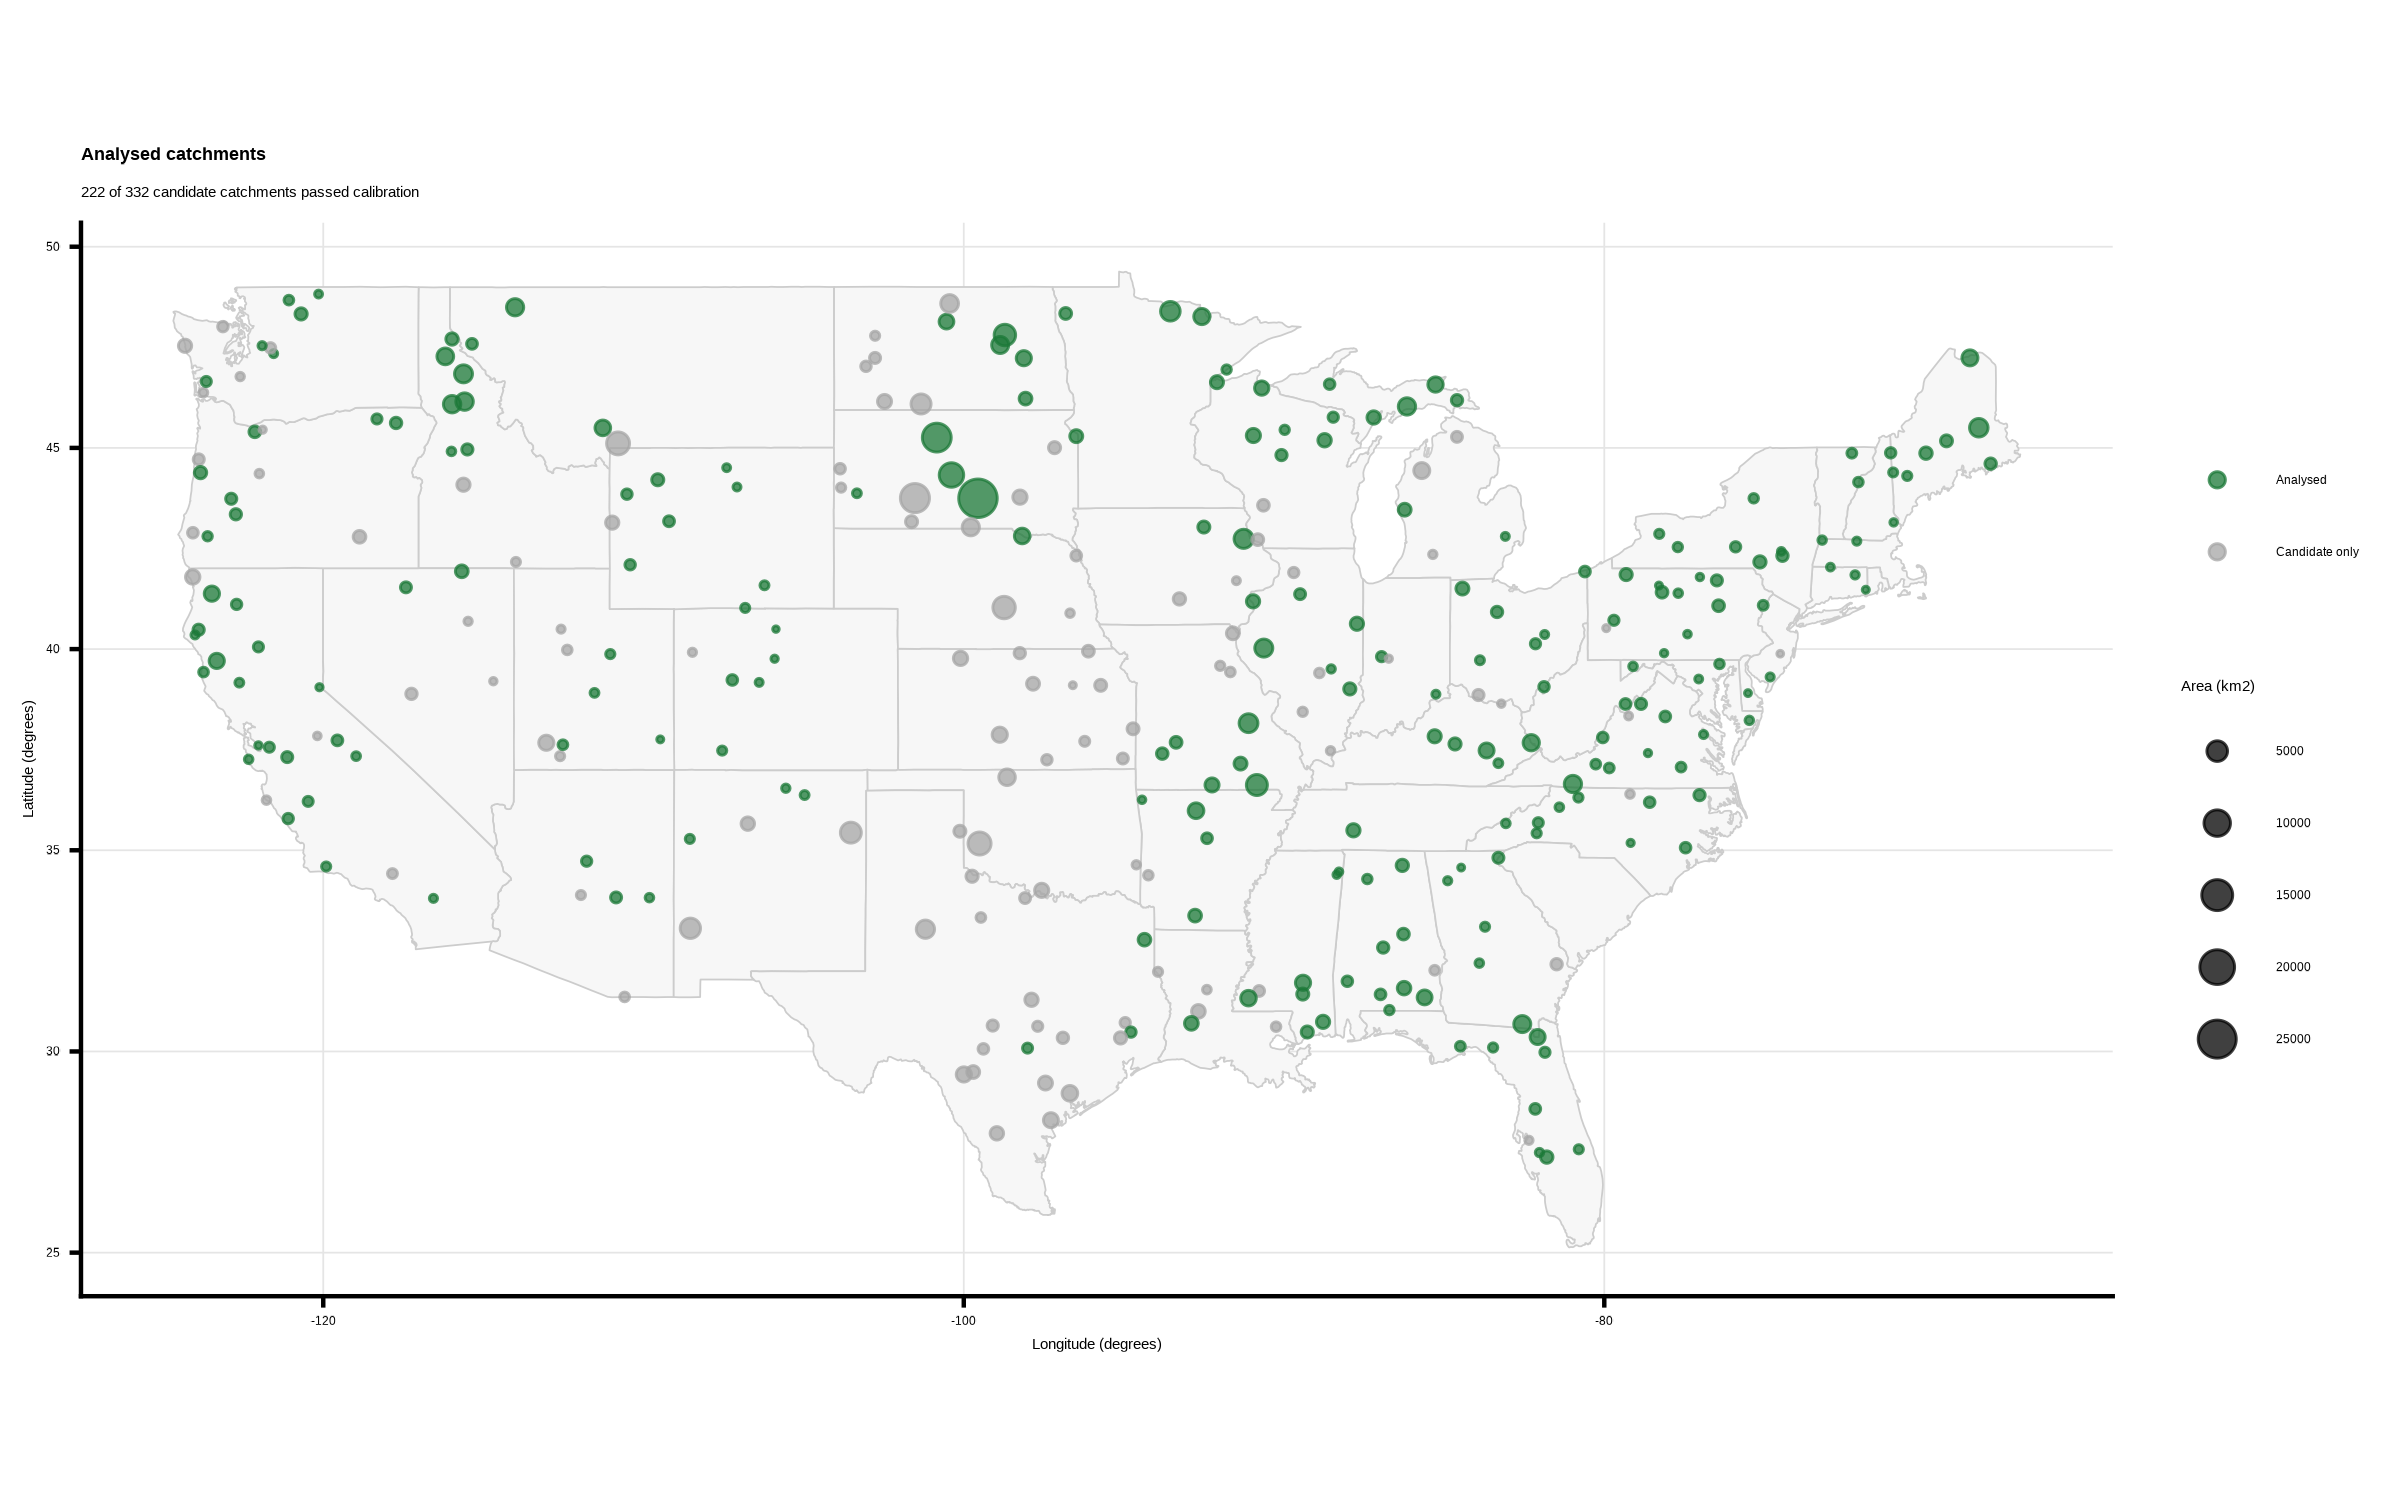
\includegraphics[width=6.26806in,height=3.91753in]{03-writeup/Revision-1/latex/media/media/image1.png}
\caption{Figure 1: Selected catchments are shown in the figure. Each
green doesn't represent the centroid of the catchment, and the size of
the dot indicates the Area (km\textsuperscript{2}) of the catchment.}
\end{figure}

The catchments used in the study are shown in Fig. 1; a total of 332
candidate catchments is selected, each circle marks the catchment
centroid and its size gives the catchment area in km2. The initial
inventory of 671 CAMELS catchments is spatially heterogeneous, with
clusters in the western and eastern United States (Fig. 2). To obtain a
representative sample for the 30-year daily simulation, the study domain
is partitioned into a uniform 1° × 1° grid and one catchment is selected
from each cell, which gives 332 candidates with even spatial coverage;
in Fig. 2 blue circles denote the full inventory and red crosses the
selected subset. For each selected catchment, daily precipitation and
minimum and maximum temperature are acquired for 1 January 1981 to 31
December 2010. Of these, the catchments that satisfy the calibration and
climate-zone requirements of Sections 3.1 and 3.2 form the analysed
sample of 222 catchments (Section 4.1).

\begin{figure}
\centering
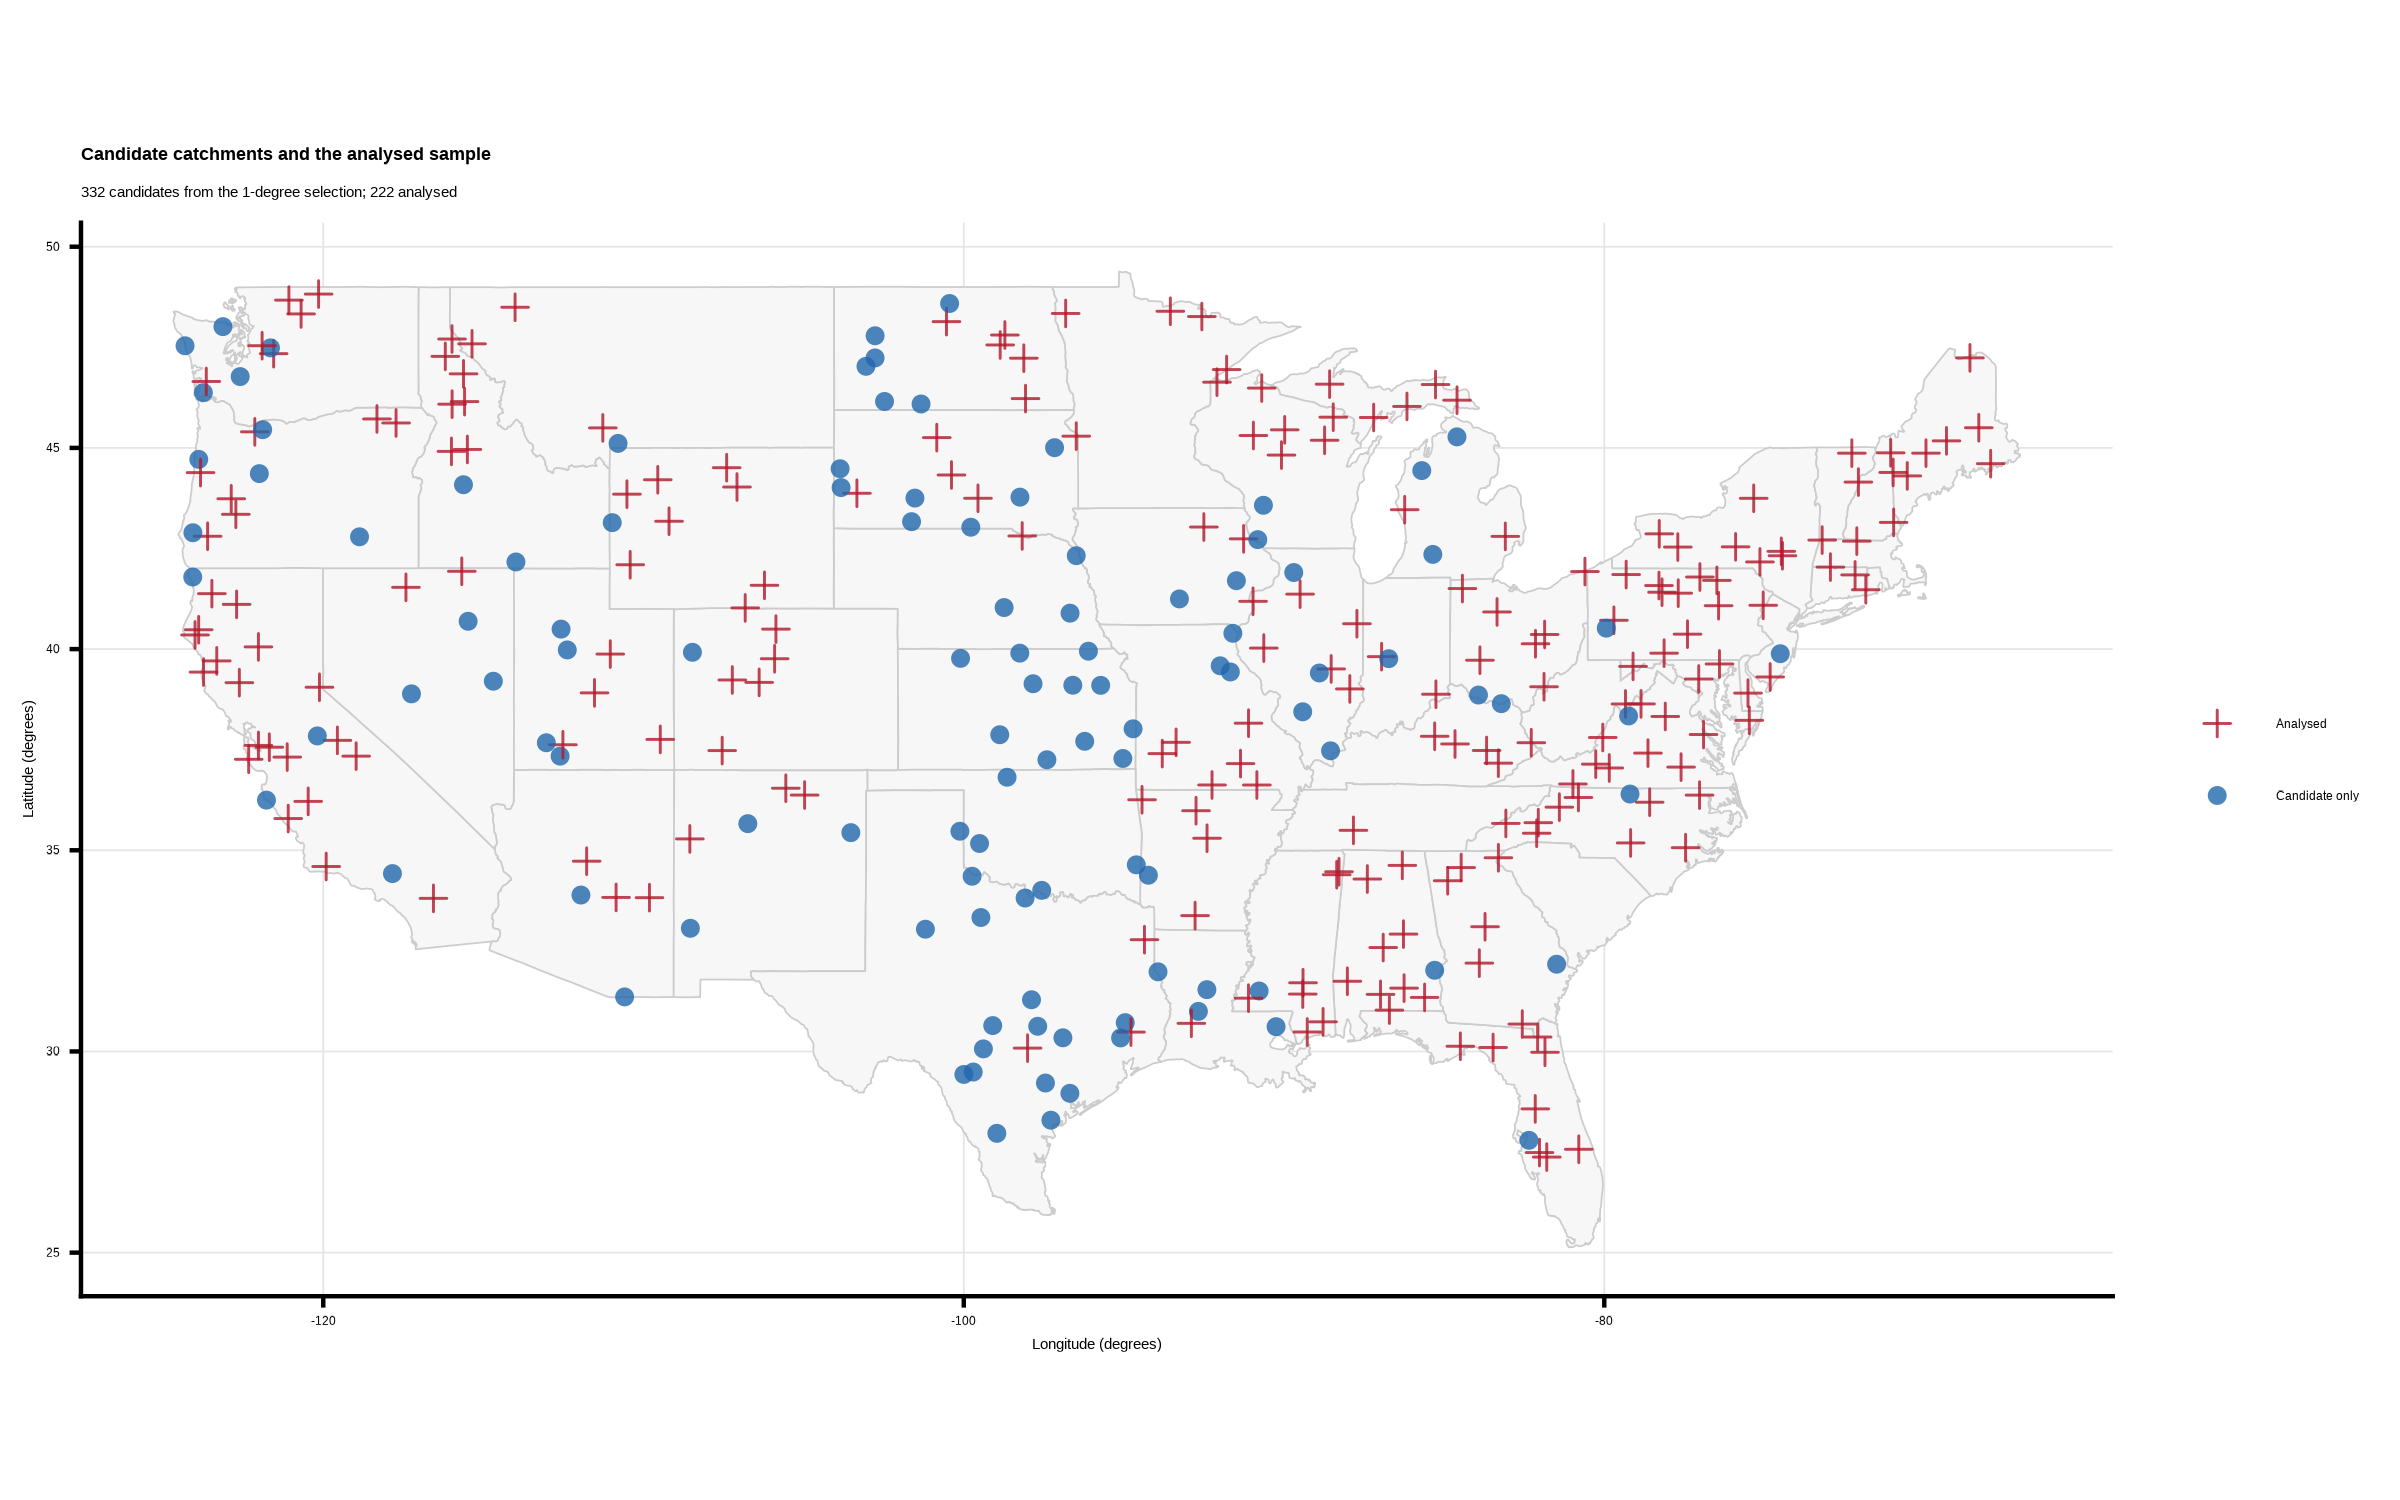
\includegraphics[width=6.26806in,height=3.91753in]{03-writeup/Revision-1/latex/media/media/image2.png}
\caption{Figure 2: Selection of catchments from all 671 catchments of
the CAMELS dataset. The blue circle shows all the catchments, and the
red cross represents the selected catchment based on the criteria for
one catchment from each 1°× 1° grid.}
\end{figure}

\section{3. Methodology}\label{methodology}

The current research establishes a comprehensive framework for
estimating catchment vulnerability to climate change, while
simultaneously combining approaches for addressing model parameter
non-stationarity through a Global Climate Zone-based methodology.
Building upon the foundational methodologies for catchment vulnerability
assessment previously developed by (Deshmukh \& Singh, 2016, 2019) the
framework conceptualizes catchment vulnerability as the critical
threshold at which climatic inputs alterations reach sufficient
magnitude to significantly modify chosen vulnerability indicators within
the critical zone. These crucial thresholds are contextualized through
specific scenarios, such as instances when a 10\% reduction in
precipitation may precipitate a corresponding 30\% decrease in
streamflow, thereby representing a condition of heightened
catchment~vulnerability. While extensive methodological approaches for
evaluating catchment vulnerabilities to climate change have been
comprehensively documented in the literature, with detailed
investigations provided by (Singh et al., 2014) and (Deshmukh \& Singh,
2016), two primary analytical paradigms have emerged: top-down and
bottom-up approaches. In contrast to traditional methodologies, the
present investigation adopts a bottom-up exploratory modeling framework
that strategically employs the Köppen-Geiger climate classification
system as a mechanistic foundation for incorporating model parameter
non-stationarity, thereby enhancing the predictive capability and
spatial applicability of vulnerability assessments across diverse
climatic regimes. In addition, the methodology employed in this study
will describe first the exploratory modeling framework and vulnerability
threshold computation in section 3.1, and then section 3.2 explains how
to integrate the model parameter non-stationarity with the Köppen-Geiger
climate classification approach.

\subsection{3.1 Exploratory Modelling Framework for Catchment
Vulnerability
Assessment}\label{exploratory-modelling-framework-for-catchment-vulnerability-assessment}

The framework originates by establishing precise descriptions of
vulnerability, which may be specified by stakeholders or water resource
managers; for example, a reduction in streamflow below a particular
threshold serves as a vulnerability criterion for the selected
catchment. Its primary objective, therefore, becomes to discover
alterations to climate and land use patterns that lead to streamflow
reductions, quantified using the exploratory modeling framework
presented in Figure 3.

The analytical approach commences by obtaining long-term time series
datasets for climatic variables, which subsequently serve as the
foundational input for scenario development. To systematically examine
potential future climatic patterns, the framework employs the delta
change methodology, wherein prospective climate scenarios are generated
through the strategic application of additive or multiplicative delta
transformations to the historical baseline data, thereby facilitating
the simulation of anticipated climate change impacts. More precisely,
scaling factors between 0.5 and 1.5 are utilized to evaluate
precipitation variability, which essentially represents systematic
deviations from the historical mean between -50\% and +50\%.
Concurrently, temperature perturbations are investigated within a range
of -2°C to +8°C compared to baseline circumstances. This comprehensive
parametric exploration enables a thorough and systematic investigation
of the potential ramifications of climate variability on streamflow
vulnerability characteristics within individual catchments, ultimately
providing robust insights into the sensitivity and robustness of
hydrological systems under diverse climatic scenarios.

\begin{figure}
\centering
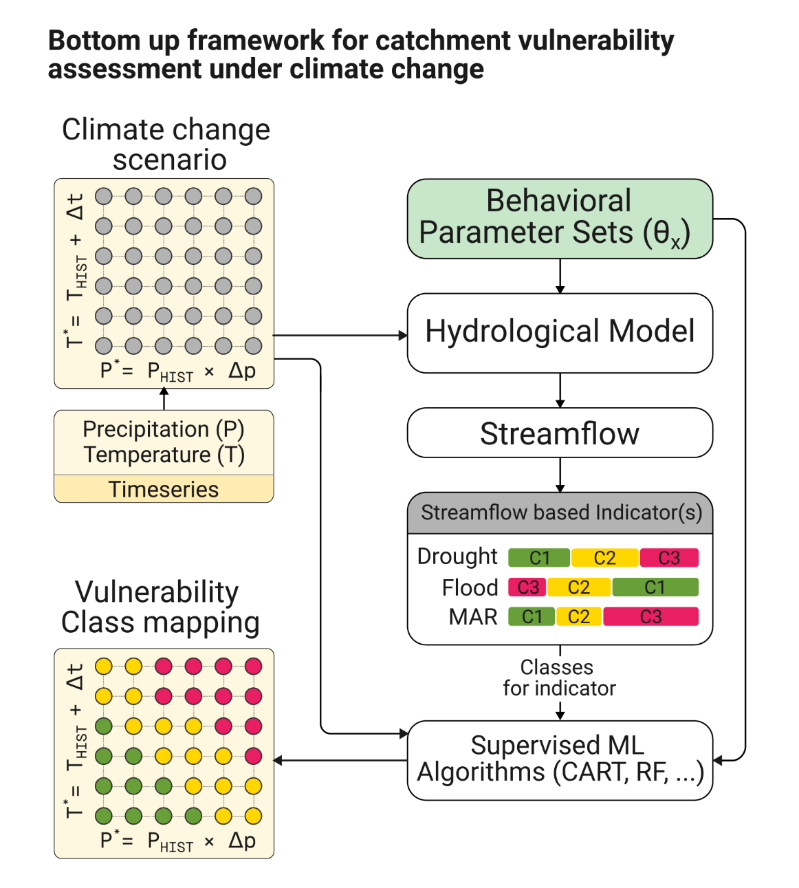
\includegraphics[width=4.12879in,height=3.82603in,alt={A diagram of a
climate change AI-generated content may be
incorrect.}]{03-writeup/Revision-1/latex/media/media/image3.png}
\caption{Figure 3 Bottom-up framework with an exploratory climate change
approach workflow to assess the catchment vulnerability.}
\end{figure}

In order to validate the hydrological model within the catchment
framework, this study employs the HBV hydrological model, developed by
(Bergström \& Forsman, 1973), later improved by (Bergström, 1995), and
finally refined by (Seibert, 1997). The combined implementation of the
HBV model utilized in this investigation indicates a conceptual
rainfall-runoff modeling framework that integrates four fundamental
hydrological processes: snow accumulation and ablation dynamics, soil
moisture accounting procedures, groundwater response mechanisms through
dual reservoir systems, and channel routing algorithms. This combined
bucket-type model architecture preserves a minimal parameter structure
with relatively modest calibration requirements while operating at daily
temporal precision and requiring a limited number of meteorological
forcing inputs, such as daily temperature, precipitation, and potential
evapotranspiration data. Consequently, the model simulates complex
hydrological processes by employing a series of interrelated computing
procedures that systematically transform meteorological inputs into
streamflow outputs via conceptual representations of catchment-scale
water storage dynamics and release mechanisms. This integrated modeling
approach offers a~thorough simulation of the complete hydrological cycle
while maintaining computational efficiency and parameter precision
required for large-scale catchment vulnerability assessments.

\begin{figure}
\centering
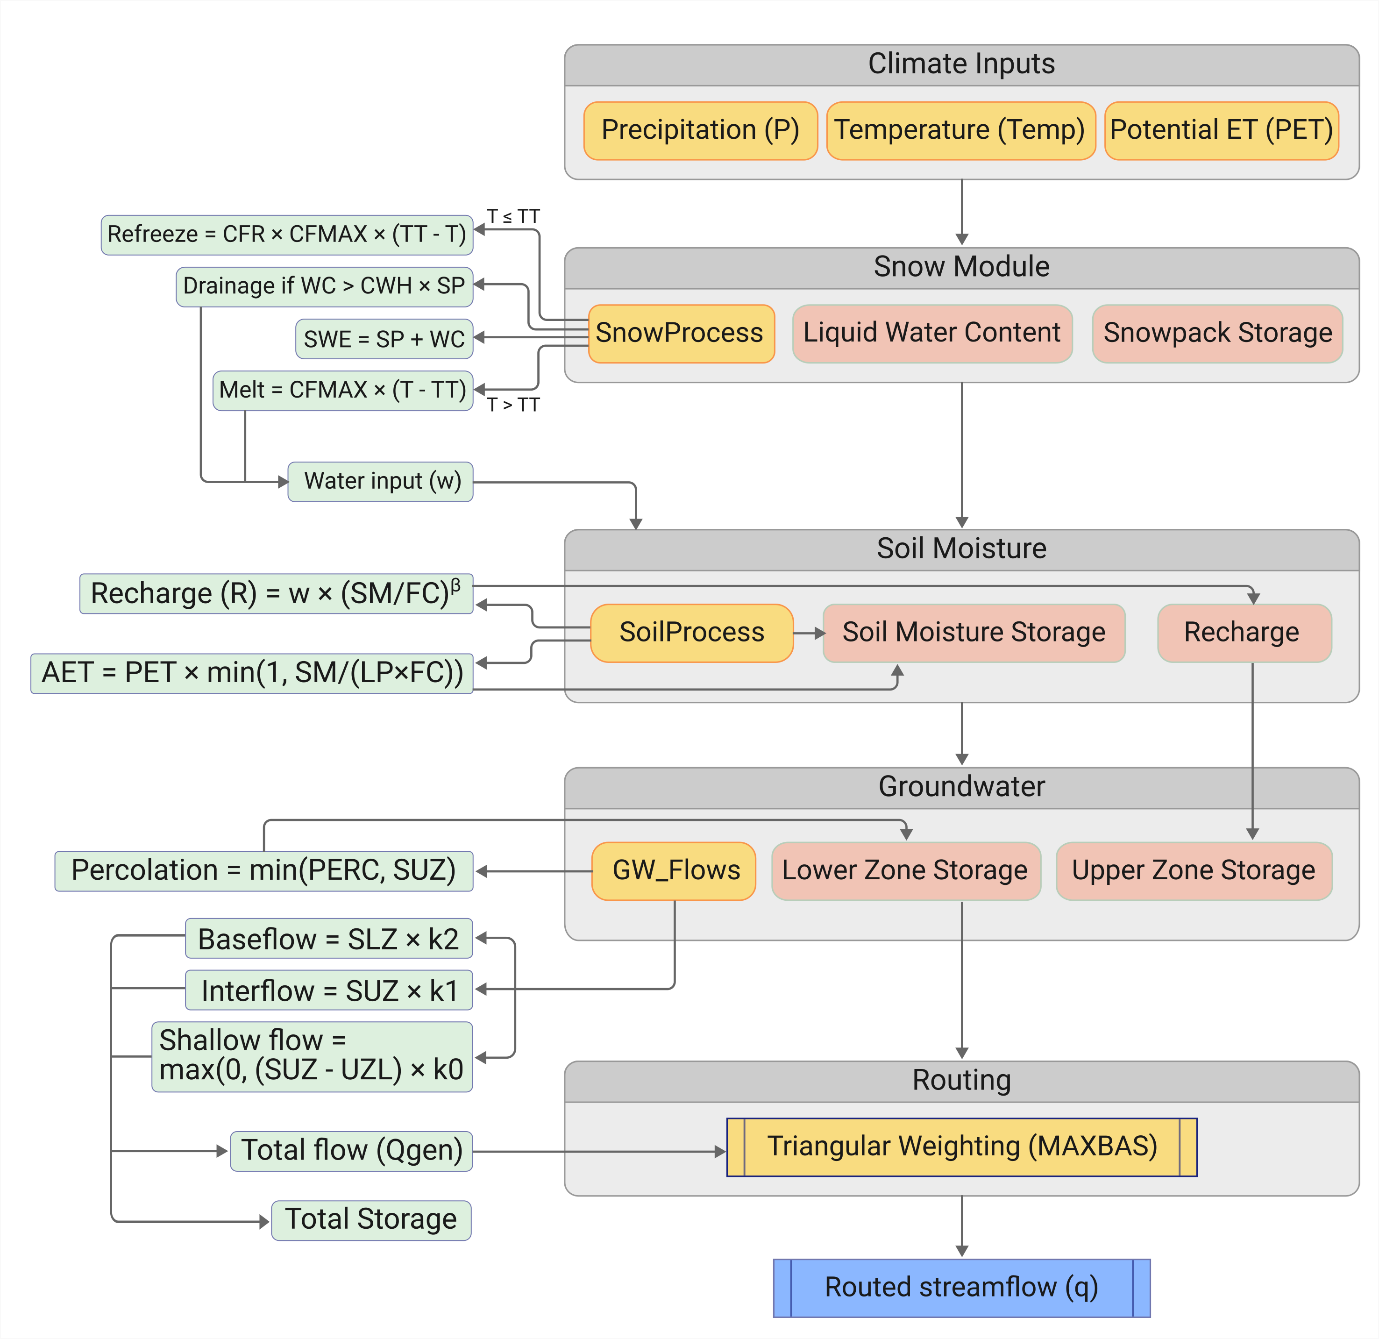
\includegraphics[width=5.37078in,height=5.21429in,alt={A diagram of a
plant AI-generated content may be
incorrect.}]{03-writeup/Revision-1/latex/media/media/image4.png}
\caption{Figure 4 Conceptual Hydrological Model Flowchart for HBV model
utilized in the study.}
\end{figure}

The HBV model is divided into discrete modules describing soil moisture
dynamics, snow accumulation and melt, and runoff generation and routing.
Each model parameter corresponds to a distinct physical or empirical
feature of catchment~hydrology. The factors FC, beta, and LP affect soil
moisture storage and evaporation processes, hence determining how
precipitation is partitioned into evapotranspiration, infiltration, and
runoff. Parameters SFCF, TT, and CFMAX provide thorough snow hydrology
modeling by differentiating between snowfall and rainfall and simulating
snowmelt through degree-day approaches adapted to local temperature
conditions. The constants k0, k1, k2, UZL, and PERC characterize
subsurface flow pathways and regression behaviors, which are critical
for distinguishing between fast and slow runoff components as well as
groundwater recharge. Lastly, MAXBAS controls the streamflow response
through routing functions that delay and smooth hydrograph peaks,
ensuring that simulated discharge coincides closely with observed flow
timing. The model parameters ranges used in the study provided in Table
2, range are majorly adopted from (Seibert, 1999; Seibert \& Vis, 2012).

\begin{longtable}[]{@{}
  >{\centering\arraybackslash}p{(\linewidth - 6\tabcolsep) * \real{0.1675}}
  >{\raggedright\arraybackslash}p{(\linewidth - 6\tabcolsep) * \real{0.0887}}
  >{\raggedright\arraybackslash}p{(\linewidth - 6\tabcolsep) * \real{0.0756}}
  >{\raggedright\arraybackslash}p{(\linewidth - 6\tabcolsep) * \real{0.6681}}@{}}
\caption{Table 2 Model Parameter Ranges used in the study for model
calibration.}\tabularnewline
\toprule\noalign{}
\begin{minipage}[b]{\linewidth}\centering
\textbf{Parameters}
\end{minipage} & \begin{minipage}[b]{\linewidth}\centering
\textbf{Min}
\end{minipage} & \begin{minipage}[b]{\linewidth}\centering
\textbf{Max}
\end{minipage} & \begin{minipage}[b]{\linewidth}\centering
\textbf{Description}
\end{minipage} \\
\midrule\noalign{}
\endfirsthead
\toprule\noalign{}
\begin{minipage}[b]{\linewidth}\centering
\textbf{Parameters}
\end{minipage} & \begin{minipage}[b]{\linewidth}\centering
\textbf{Min}
\end{minipage} & \begin{minipage}[b]{\linewidth}\centering
\textbf{Max}
\end{minipage} & \begin{minipage}[b]{\linewidth}\centering
\textbf{Description}
\end{minipage} \\
\midrule\noalign{}
\endhead
\bottomrule\noalign{}
\endlastfoot
FC & 40 & 400 & Maximum soil moisture storage, field capacity \\
beta & 1 & 6 & Shape coefficient governing fate of water input to soil
moisture storage \\
LP & 0.3 & 1 & Threshold for reduction of evaporation \\
SFCF & 0.4 & 1.2 & Snowfall correction factor \\
TT & -2.5 & 2.5 & Threshold temperature \\
CFMAX & 1 & 8 & Degree-day factor \\
k0 & 0.05 & 0.5 & Recession constant (upper storage, near surface) \\
k1 & 0.01 & 0.3 & Recession constant (upper storage) \\
k2 & 0.001 & 0.15 & Recession constant (lower storage) \\
UZL & 0 & 70 & Threshold for shallow storage \\
PERC & 0 & 4 & Percolation, max flow from upper to lower storage \\
MAXBAS & 1 & 3 & Base of the triangular routing function (in days) \\
\end{longtable}

To produce the parameter sets for hydrological model response
simulation, Latin Hypercube Sampling (LHS) is utilized as a stratified
Monte Carlo sampling approach. This ensures consistent and organized
coverage throughout the distribution space of each parameter. Unlike
typical random sampling procedures, LHS precisely partitions each
parameter\textquotesingle s range into \(n\) equiprobable strata for
\(n\) samples, subsequently selecting exactly one sample from each
stratum before randomly integrating these samples across parameters to
generate coherent parameter sets. The LHS provides significantly better
coverage of the multidimensional parameter space compared to uniform
random sampling designs, making it particularly advantageous when
parameter-specified values are computationally restricted. The generated
parameter sets are used is used in conjunction with climatic~time series
data to simulate catchment runoff responses and, the simulated runoff
evaluated against observed discharge data using established performance
metrics, including the Kling-Gupta Efficiency (KGE), Nash-Sutcliffe
Efficiency (NSE), and percentage bias (PBIAS), to systematically
identify behavioral parameter sets. This validation method subsequently
permits the selection of the 200 best-ranked behavioural parameter sets
per catchment (\(\theta_{x}\)) based on these comprehensive performance
indicators. The aforementioned methodology is explained in Fig. 5 where
model is calibrated, and behavioral parameter sets are identified.

\begin{figure}
\centering
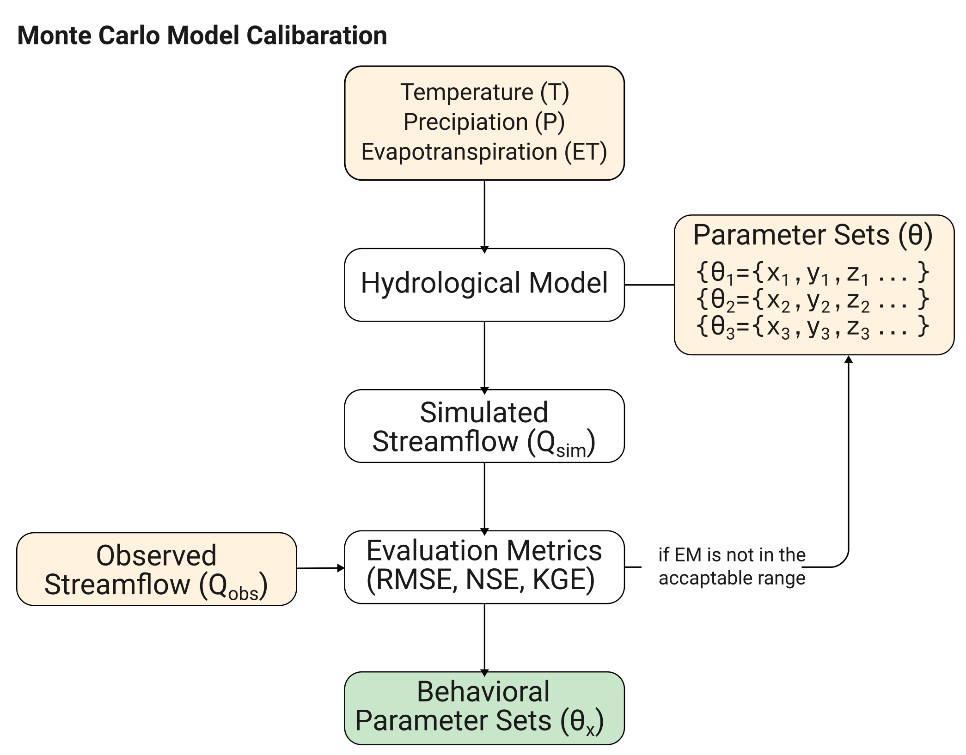
\includegraphics[width=4.37083in,height=3.19335in,alt={A diagram of a
model AI-generated content may be
incorrect.}]{03-writeup/Revision-1/latex/media/media/image5.png}
\caption{Figure 5: Methodology adopted for the hydrological model using
Monte-Carlo Calibration.}
\end{figure}

To simulate runoff efficiently, potential evapotranspiration (PET) data
is essential. Although the long-term historical PET data is provided by
CAMELS dataset, but study required the methodology to compute PET time
series as the climate change induced using delta change method. The
present investigation explored two widely used methods for PET
estimation, the Hamon and Hargreaves approaches, because of~their
relatively simple data requirements, which consist of simply daily
minimum and maximum temperatures coupled with latitude information.
According to (Lu et al., 2005), the Hamon approach demonstrates higher
accuracy in circumstances characterized by minimal temperature
variability, notably in regions with sufficient water availability.
Conversely, in regions exhibiting substantial variations in temperature,
the Hargreaves approach is regarded as a more reliable estimator. The
Hargreaves approach is applied to model PET development for all climatic
circumstances. The equation (1) computes the PET in mm/day, where the
daily minimum, maximum, and mean temperatures are supplied in degrees
Celsius. The 0.408 MJ m−2 d−1 latent-heat conversion is applied so that
the radiation term is expressed in mm d−1, and PET is recomputed for
every perturbed climate scenario. In this equation, \(R_{a}\) represents
the extra-terrestrial radiation in mm/day, which varies with latitude
and the day of the year, and is computed by the equation (2), given the
constant \(G_{s}\) is the solar constant (0.0820 MJ/m2/min).

{\def\LTcaptype{none} % do not increment counter
\begin{longtable}[]{@{}
  >{\raggedright\arraybackslash}p{(\linewidth - 4\tabcolsep) * \real{0.0907}}
  >{\raggedright\arraybackslash}p{(\linewidth - 4\tabcolsep) * \real{0.8071}}
  >{\raggedright\arraybackslash}p{(\linewidth - 4\tabcolsep) * \real{0.1022}}@{}}
\toprule\noalign{}
\begin{minipage}[b]{\linewidth}\raggedright
\end{minipage} & \begin{minipage}[b]{\linewidth}\raggedright
\[\text{PET} = 0.0023 \times \left( T_{\text{mean}} + 17.8 \right) \times \left( T_{\text{max}} - T_{\text{min}} \right)^{0.5} \times R_{a}\]
\end{minipage} & \begin{minipage}[b]{\linewidth}\raggedright
(1)
\end{minipage} \\
\midrule\noalign{}
\endhead
\bottomrule\noalign{}
\endlastfoot
\end{longtable}
}

{\def\LTcaptype{none} % do not increment counter
\begin{longtable}[]{@{}
  >{\raggedright\arraybackslash}p{(\linewidth - 4\tabcolsep) * \real{0.0309}}
  >{\raggedright\arraybackslash}p{(\linewidth - 4\tabcolsep) * \real{0.8758}}
  >{\raggedright\arraybackslash}p{(\linewidth - 4\tabcolsep) * \real{0.0933}}@{}}
\toprule\noalign{}
\begin{minipage}[b]{\linewidth}\raggedright
\end{minipage} & \begin{minipage}[b]{\linewidth}\raggedright
\[R_{a} = \frac{24 \times 60}{\pi} \times G_{s} \times d_{r} \times \left\lbrack \omega_{s} \times \sin\left( \text{lat} \right) \times \sin(\delta) + \cos\left( \text{lat} \right) \times \cos(\delta) \times \sin\left( \omega_{s} \right) \right\rbrack\]
\end{minipage} & \begin{minipage}[b]{\linewidth}\raggedright
(2)
\end{minipage} \\
\midrule\noalign{}
\endhead
\bottomrule\noalign{}
\endlastfoot
\end{longtable}
}

where, \(d_{r}\) is the inverse relative distance between the Earth and
the Sun, which can be descibed as
\(d_{r} = 1 + 0.033 \times \cos\left( \frac{2\pi d}{365} \right)\) and
\emph{d} is the Julian day. Also, \emph{ω\textsubscript{s}} is the
sunset hour angle, computed using the expression
\(\omega_{s} = \arccos\left( - \tan\left( \text{lat} \right) \times \tan(\delta) \right)\)
and \emph{δ} is the solar declination angle, calculated by
\(\delta = 0.409 \times \sin\left( \frac{2\pi d}{365} - 1.39 \right)\).

The Nash--Sutcliffe Efficiency (NSE), the Kling--Gupta Efficiency (KGE),
and the Percent Bias (PBIAS) model performance measures are applied to
compare simulated outcomes (\emph{S\textsubscript{i}}) over observed
records (\emph{O\textsubscript{i}}) across \(n\) time steps employing a
variety of quantitative statistical metrics (Althoff \& Rodrigues, 2021;
Cinkus et al., 2023; Moriasi et al., 2007). The Nash--Sutcliffe
Efficiency (NSE) determines the degree of agreement between simulations
and observations by comparing the sum of squared model errors to the sum
of squared deviations of the observations from their mean
\(\overline{O}\) (Nash \& Sutcliffe, 1970) (cf. equation 3). Its values
can range from \(- \infty\) to \(1\), with \(1\) representing a perfect
match, \(0\) signifying performance identical to the mean observation,
and negative values implying performance inferior to~the observational
mean. Despite being widely utilized, NSE is vulnerable to outliers and,
because of its primary emphasis on peak flows, has an ability to
over-penalize underpredictions of extreme events.

{\def\LTcaptype{none} % do not increment counter
\begin{longtable}[]{@{}
  >{\raggedright\arraybackslash}p{(\linewidth - 4\tabcolsep) * \real{0.0904}}
  >{\raggedright\arraybackslash}p{(\linewidth - 4\tabcolsep) * \real{0.8165}}
  >{\raggedright\arraybackslash}p{(\linewidth - 4\tabcolsep) * \real{0.0931}}@{}}
\toprule\noalign{}
\begin{minipage}[b]{\linewidth}\raggedright
\end{minipage} & \begin{minipage}[b]{\linewidth}\centering
\[\text{NSE} = 1 - \frac{\sum_{i = 1}^{n}\left( O_{i} - S_{i} \right)^{2}}{\sum_{i = 1}^{n}\left( O_{i} - \overline{O} \right)^{2}}\]
\end{minipage} & \begin{minipage}[b]{\linewidth}\raggedright
(3)
\end{minipage} \\
\midrule\noalign{}
\endhead
\bottomrule\noalign{}
\endlastfoot
\end{longtable}
}

The Kling--Gupta Efficiency (KGE) (Gupta et al., 2009) offers a more
thoroughly balanced evaluation by dividing model performance into three
components: linear correlation (\(r\)), bias ratio (\(\beta\)), and
variability ratio (\(\gamma\)) (c.f. equation 4). This formulation
provides simultaneous assessment of accuracy in correlation, magnitude,
and variability, with an optimum value of 1 representing total
convergence. KGE is often less sensitive to extremes than NSE but may be
more challenging to figure out.

{\def\LTcaptype{none} % do not increment counter
\begin{longtable}[]{@{}
  >{\raggedright\arraybackslash}p{(\linewidth - 4\tabcolsep) * \real{0.0894}}
  >{\raggedright\arraybackslash}p{(\linewidth - 4\tabcolsep) * \real{0.8189}}
  >{\raggedright\arraybackslash}p{(\linewidth - 4\tabcolsep) * \real{0.0917}}@{}}
\toprule\noalign{}
\begin{minipage}[b]{\linewidth}\raggedright
\end{minipage} & \begin{minipage}[b]{\linewidth}\centering
\[\text{KGE} = 1 - \sqrt{(r - 1)^{2} + (\beta - 1)^{2} + (\gamma - 1)^{2}}\]
\end{minipage} & \begin{minipage}[b]{\linewidth}\raggedright
(4)
\end{minipage} \\
\midrule\noalign{}
\endhead
\bottomrule\noalign{}
\endlastfoot
\end{longtable}
}

The Percent Bias (PBIAS) indicator evaluates the average tendency of
simulations to over- or underestimate observations, represented as a
percentage deviation of the simulated mean from the observed mean (cf.
equation 5). An optimal PBIAS value is 0\%, with positive values
indicating underestimation and negative values indicating
overestimation. While it presents a fundamental overview of systematic
water balance challenges, PBIAS does not account for timing or
variability inconsistencies.

{\def\LTcaptype{none} % do not increment counter
\begin{longtable}[]{@{}
  >{\raggedright\arraybackslash}p{(\linewidth - 4\tabcolsep) * \real{0.0905}}
  >{\raggedright\arraybackslash}p{(\linewidth - 4\tabcolsep) * \real{0.8172}}
  >{\raggedright\arraybackslash}p{(\linewidth - 4\tabcolsep) * \real{0.0923}}@{}}
\toprule\noalign{}
\begin{minipage}[b]{\linewidth}\raggedright
\end{minipage} & \begin{minipage}[b]{\linewidth}\centering
\[\text{PBE} = \frac{\sum_{i = 1}^{n}\left( O_{i} - S_{i} \right)}{\sum_{i = 1}^{n}O_{i}} \times 100\%\]
\end{minipage} & \begin{minipage}[b]{\linewidth}\raggedright
(5)
\end{minipage} \\
\midrule\noalign{}
\endhead
\bottomrule\noalign{}
\endlastfoot
\end{longtable}
}

Further, for the model calibration procedure, limiting PBIAS to
\(\pm 25\%\) and KGE ≥ 0.5, then simulate streamflow for 10,000 Latin
hypercube parameter combinations. NSE is reported but is not used to
screen, and the 200 best-ranked behavioural sets are retained per
catchment. Catchments that do not produce at least 50 behavioural
parameter sets are excluded. Table 3 reports the calibration performance
and Table 4 the split-sample results. Calibration uses 1981--2010 with a
two-year warm-up; temporal transferability is tested separately with
forward and reverse split-sample experiments and ten-year moving windows
(Shen et al., 2022).

The main objective of the present investigation focuses on the mean
annual runoff (MAR) indicator (MA\_41) cf. (Olden \& Poff, 2003). This
indicates mean flow conditions and is implemented as the mean annual
runoff (MAR), defined as the ratio of the mean annual discharge to the
catchment area, thereby normalizing runoff with respect to basin size.
MAR utilized to determining hydrological vulnerability classes with
respect to streamflow reductions within the catchment. Vulnerability is
defined according to differences from long-term historical runoff: Class
0 signifies no vulnerability and corresponds to no change or to a change
in the non-vulnerable direction; Class 1 is a change of up to 25\% in
the vulnerable direction; Class 2 is a change of 25 to 50\%; and Class 3
is a change exceeding 50\%. The same four-class scale is applied to two
further indicators: the low-flow index (LFI, mean annual minimum divided
by mean annual mean) and the high-flow ratio (MAMF, median annual
maximum divided by median annual median). A decrease is treated as the
vulnerable direction for MAR and LFI, and an increase for MAMF, because
an increase in MAMF represents intensification of high flows. MAR is the
primary indicator; LFI and MAMF are reported alongside it to test
whether the conclusions depend on the chosen indicator.

Once the indicator's vulnerability classes are identified, the following
stage is to find the climate change thresholds (precipitation,
temperature, land use, etc.) that may lead the indicator to a particular
vulnerability class. In most cases, it is~necessary to determine the
most vulnerable class (Class-3 in the case of MAR in this study), which
is estimated by mapping the change in climate scenarios to the indicator
classes. The proposed investigation estimates the threshold from the
prevalence of the most vulnerable class, using an isotonic regression on
the marginal prevalence curve and a logistic model on the precipitation
and temperature perturbations, with a classification and regression tree
(CART) (Breiman et al., 1984) used as an independent cross-check that
maps the perturbed precipitation and temperature to indicator classes.
In addition, the CART algorithm is a recursive partitioning approach for
supervised learning challenges involving both classification and
regression. By iteratively dividing the dataset according to predictor
variables, selecting split points that maximize a given impurity
criterion, the Gini impurity for classification, and least-squares error
for regression, the technique creates a binary decision tree. At each
node, the method examines all possible partitions across candidate
variables to discover the section that produces the greatest reduction
in impurity, adopting a greedy search heuristic. The tree growth
continues until predetermined stopping criteria, such as minimum node
size or maximum tree depth, are fulfilled (Therneau et al., 2019).

The selection of the vulnerability threshold therefore reduces to
estimating the magnitude of climatic change that makes the most
vulnerable class (Class 3) the most likely outcome for the selected
indicator. A typical CART result, which classifies indicator
vulnerability classes from delta changes in temperature and
precipitation and from model parameters, is shown in Fig. 6. The tree
started at a single root node, wherein the entire dataset is partitioned
according to a threshold criterion applied to the inputs (\(dp\), \(dt\)
and parameters). Each subsequent internal node executes a binary split,
leading observations either left or right based on whether the
associated feature value satisfies the specified threshold. This
continuous bifurcation continues until terminal nodes (leaves) are
reached, which assign the final class labels. The cross-check weights
each terminal node by its sample size, so that the reported values
reflect the relative prevalence of the most vulnerable class in the
tree, for detailed understanding the vulnerability threshold computation
for precipitation and temperature check (Deshmukh \& Singh, 2016).

\begin{figure}
\centering
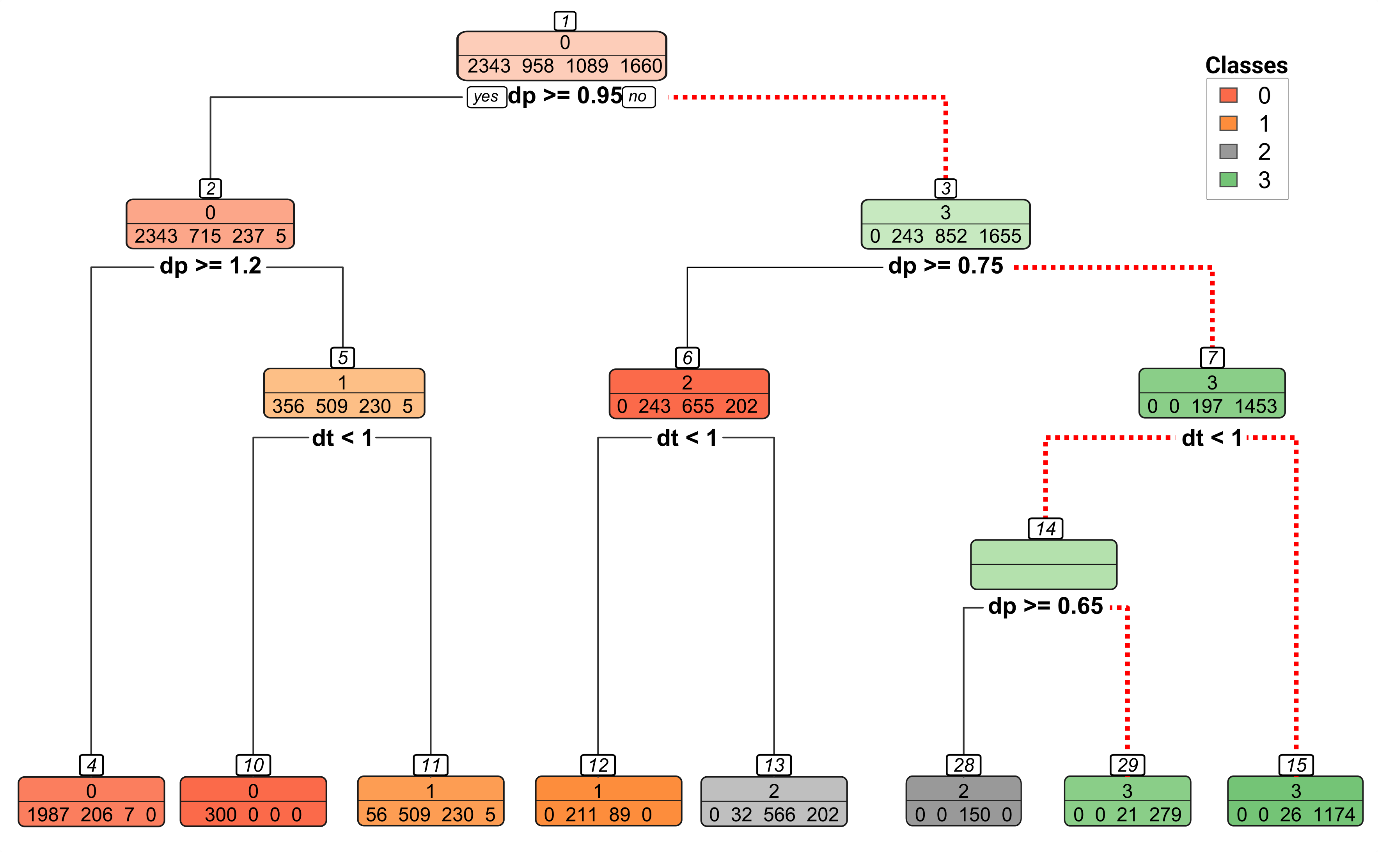
\includegraphics[width=6.26806in,height=3.87292in]{03-writeup/Revision-1/latex/media/media/image6.png}
\caption{Figure 6: Binary tree classification of class distribution for
MAR for catchment (USID: 01439500). The path of the most vulnerable
class is shown with the dashed red line.}
\end{figure}

\emph{The procedure described above for determining catchment
vulnerability thresholds for precipitation and temperature under climate
change constitutes what we term the~\textbf{Stationary Parameter
Framework (SPF)}. This approach does not incorporate climate
change-induced parameter non-stationarity, as behavioral parameter sets
remain fixed throughout all climate scenarios, assuming temporal
invariance of model parameters.}

The method demonstrated above for establishing catchment vulnerability
thresholds for precipitation and temperature in the context of climate
change is referred to as the Stationary Parameter Framework (SPF). This
methodology does not account for non-stationarity of parameters by
climate change, as the behavioural parameter sets are maintained
constant across all climate scenarios, supposing temporal invariance of
model parameters.

\subsection{\texorpdfstring{3.2 Climate Zone-Informed Parameter
Evolution Framework (CZIPEF) for catchment vulnerability assessment
under climate change
}{3.2 Climate Zone-Informed Parameter Evolution Framework (CZIPEF) for catchment vulnerability assessment under climate change }}\label{climate-zone-informed-parameter-evolution-framework-czipef-for-catchment-vulnerability-assessment-under-climate-change}

The procedure used to determine the catchment vulnerability threshold
for precipitation and temperature under climate change is shown in the
previous section, and the vulnerability thresholds are computed
employing the specified approach, which does not incorporate the climate
change-based parametric stationarity. To incorporate not stationarity in
the vulnerability quantification, the study employs the Köppen-Geiger
climate classification to sample the new parameter sets if the
catchment\textquotesingle s climate zone changes due to climate change.

The Köppen-Geiger climate classification constitutes one of the most
widely recognized and widely utilized frameworks for categorizing the
varied climatic regimes across the globe. The five primary categories of
terrestrial climates are tropical (\(A\)), arid (\(B\)), temperate
(\(C\)), cold or continental (\(D\)), and polar (\(E\)). These are
further subdivided based on particular patterns of temperature and
precipitation seasonality. This system was first developed by
climatologist Wladimir Köppen in the late nineteenth century and later
improved by Rudolf Geiger (Beck et al., 2023; Peel et al., 2007), the
classes are shown in the Table 1. The scientific foundation of the
Köppen-Geiger classification system lies in its exceptional correlation
with global vegetation and ecosystem distributions. This concept is
based on the principle that climatic factors, primarily air temperature
and precipitation, are the fundamental drivers determining large-scale
biogeographical patterns. By applying particular threshold values for
temperature and precipitation, the Köppen-Geiger method produces
climatic zones that approximately correlate to the natural distribution
of the primary vegetation types. Consequently, it offers an ecologically
appropriate framework that is frequently employed in environmental,
hydrological, and ecological investigations, as well as in impact of
climate change assessments.

To incorporate model parametric non-stationarity resulting from a
catchment's shift in its historical Köppen-Geiger classification due to
climate change, behavioral parameter sets are sampled again from pooled
parameter sets corresponding to the catchment's updated Köppen-Geiger
climate zone, for example, catchments historical climate zone is Cfa and
after applying climate change the new climate change is BSk then for
this particular climate change case parameter sets will be sampled from
BSk corresponding pooled parameter sets. The resampling process and
establishing behavioral parameters for each potential Köppen-Geiger
Class appropriate to the study area is presented in Figure 7. The

\begin{figure}
\centering
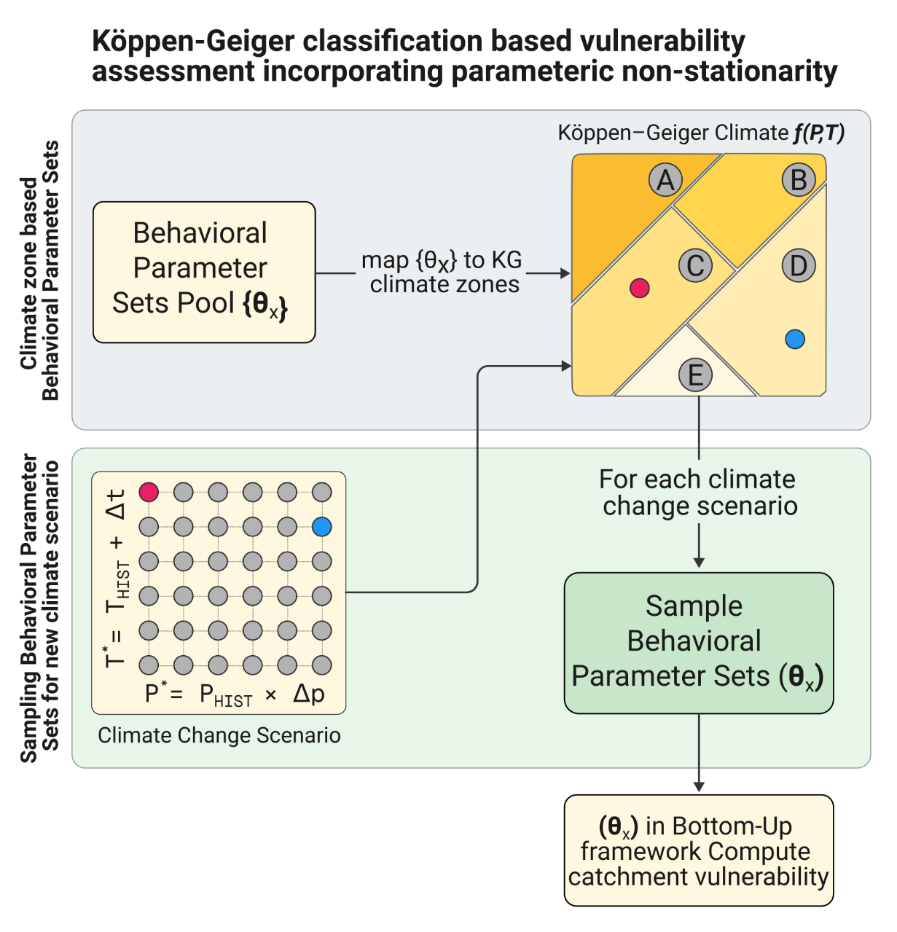
\includegraphics[width=4.06181in,height=3.80557in,alt={A diagram of a
climate change scenario AI-generated content may be
incorrect.}]{03-writeup/Revision-1/latex/media/media/image7.png}
\caption{Figure 7: The flowchart explains the incorporation of the
Köppen-Geiger climate classification with an exploratory modelling
framework. After mapping behavioral parameter sets to the climate
classification and resampling from the parameters of the catchment show
the climate change is shown under synthetic climate cases.}
\end{figure}

For each analysed catchment, the retained behavioural parameter sets
are~initially identified. Catchments are~then categorized according to
their historical Köppen-Geiger climate zones, and the behavioral
parameter sets within each zone were pooled to produce climate
zone--specific behavioral parameter datasets.

New parameter sets are drawn from the destination climate zone with a
Gaussian copula fitted to the pooled behavioural sets: the empirical
marginal distribution of each parameter is preserved, the rank
correlation between parameters is retained, and every draw is bounded by
the parameter ranges in Table 2. A univariate kernel density estimator
was also considered but is not used, because it ignores the correlation
between parameters and can produce out-of-range values. The KDE of a set
of \(n\) data points \((x_{1},x_{2},\ldots,x_{n})\) is defined by
equation 6, where the estimated density at point \(x\) is represented by
\(\hat{f}(x)\), \(n\) means the number of data points, \(h\) denotes the
bandwidth or smoothing parameter, and \(K( \cdot )\) is a kernel
function that determines the shape of the curve at each data point.

{\def\LTcaptype{none} % do not increment counter
\begin{longtable}[]{@{}
  >{\raggedright\arraybackslash}p{(\linewidth - 4\tabcolsep) * \real{0.0902}}
  >{\raggedright\arraybackslash}p{(\linewidth - 4\tabcolsep) * \real{0.8168}}
  >{\raggedright\arraybackslash}p{(\linewidth - 4\tabcolsep) * \real{0.0931}}@{}}
\toprule\noalign{}
\begin{minipage}[b]{\linewidth}\raggedright
\end{minipage} & \begin{minipage}[b]{\linewidth}\raggedright
\[\hat{f}(x) = \frac{1}{nh}\sum_{i = 1}^{n}{K\left( \frac{x - x_{i}}{h} \right)}\]
\end{minipage} & \begin{minipage}[b]{\linewidth}\raggedleft
(6)
\end{minipage} \\
\midrule\noalign{}
\endhead
\bottomrule\noalign{}
\endlastfoot
\end{longtable}
}

Moreover, for each climate change prediction, model parameters are
estimated from the pool of the destination climate zone, and the three
flow indicators are computed to characterize non-stationarity in
catchment responses. Vulnerability thresholds for precipitation and
temperature are then estimated with isotonic and logistic prevalence
models for each catchment, framework and indicator, with binomial
bootstrap intervals (Section 3.1).

\section{4. Results}\label{results}

A comparative investigation of change in vulnerability thresholds under
climate change is performed by comparing the Stationary Parameter
Framework (SPF) with the Climate Zone-Informed Parameter Evolution
Framework (CZIPEF). The synthetic climate is constructed with the
delta-change method applied to the observed 1981-2010 series:
precipitation is multiplied by 0.5 to 1.5 in steps of 0.1 and
temperature is shifted by -2 to +8 °C in 1 °C steps, which gives 121
combinations per catchment. Every combination is reclassified with the
Beck et al. (2023) scheme applied to the perturbed monthly climate
normals. Fig. 8 maps the resulting classes for precipitation multipliers
of 0.5, 1.0 and 1.5 crossed with warming of +1.5, +2, +3 and +4 °C, and
Table 5b summarises how many catchments change class at each level. At
+4 °C, 50\% of catchments change class without a precipitation change,
58\% under a 50\% reduction and 51\% under a 50\% increase; at +1.5 °C
the corresponding shares are 16\%, 30\% and 19\%. At +2 °C between 16\%
and 37\% of catchments change class depending on the precipitation
multiplier, against 50-58\% at +4 °C.

The synthetic scenarios produce a range of climatic classifications
across the analysed catchments. Observed decadal reclassification is
reported separately from the synthetic scenarios (Table 5): 21\% of
catchments record at least one change of class between 1981-1990,
1991-2000 and 2001-2010, while most retain their baseline class across
the three decades. Under the synthetic scenarios 92\% of catchments
change class in at least one of the 121 combinations, and the median
catchment visits three classes. Some scenarios move a catchment into a
class that has no pool of behavioural parameter sets: no analysed
catchment falls in Af, Am, Aw, BSh, BWh or BWk in the baseline period,
so these classes have no pool. Such scenarios are flagged as fallbacks,
keep the baseline parameter sets and are excluded when the thresholds
are estimated; catchments in which more than 10\% of scenarios fall back
are reported separately. After this filtering, 222 of the 332 candidate
catchments remain for further study: those that produced at least 50
behavioural parameter sets under KGE ≥ 0.5 and \textbar PBIAS\textbar{}
≤ 25\%.

\begin{figure}
\centering
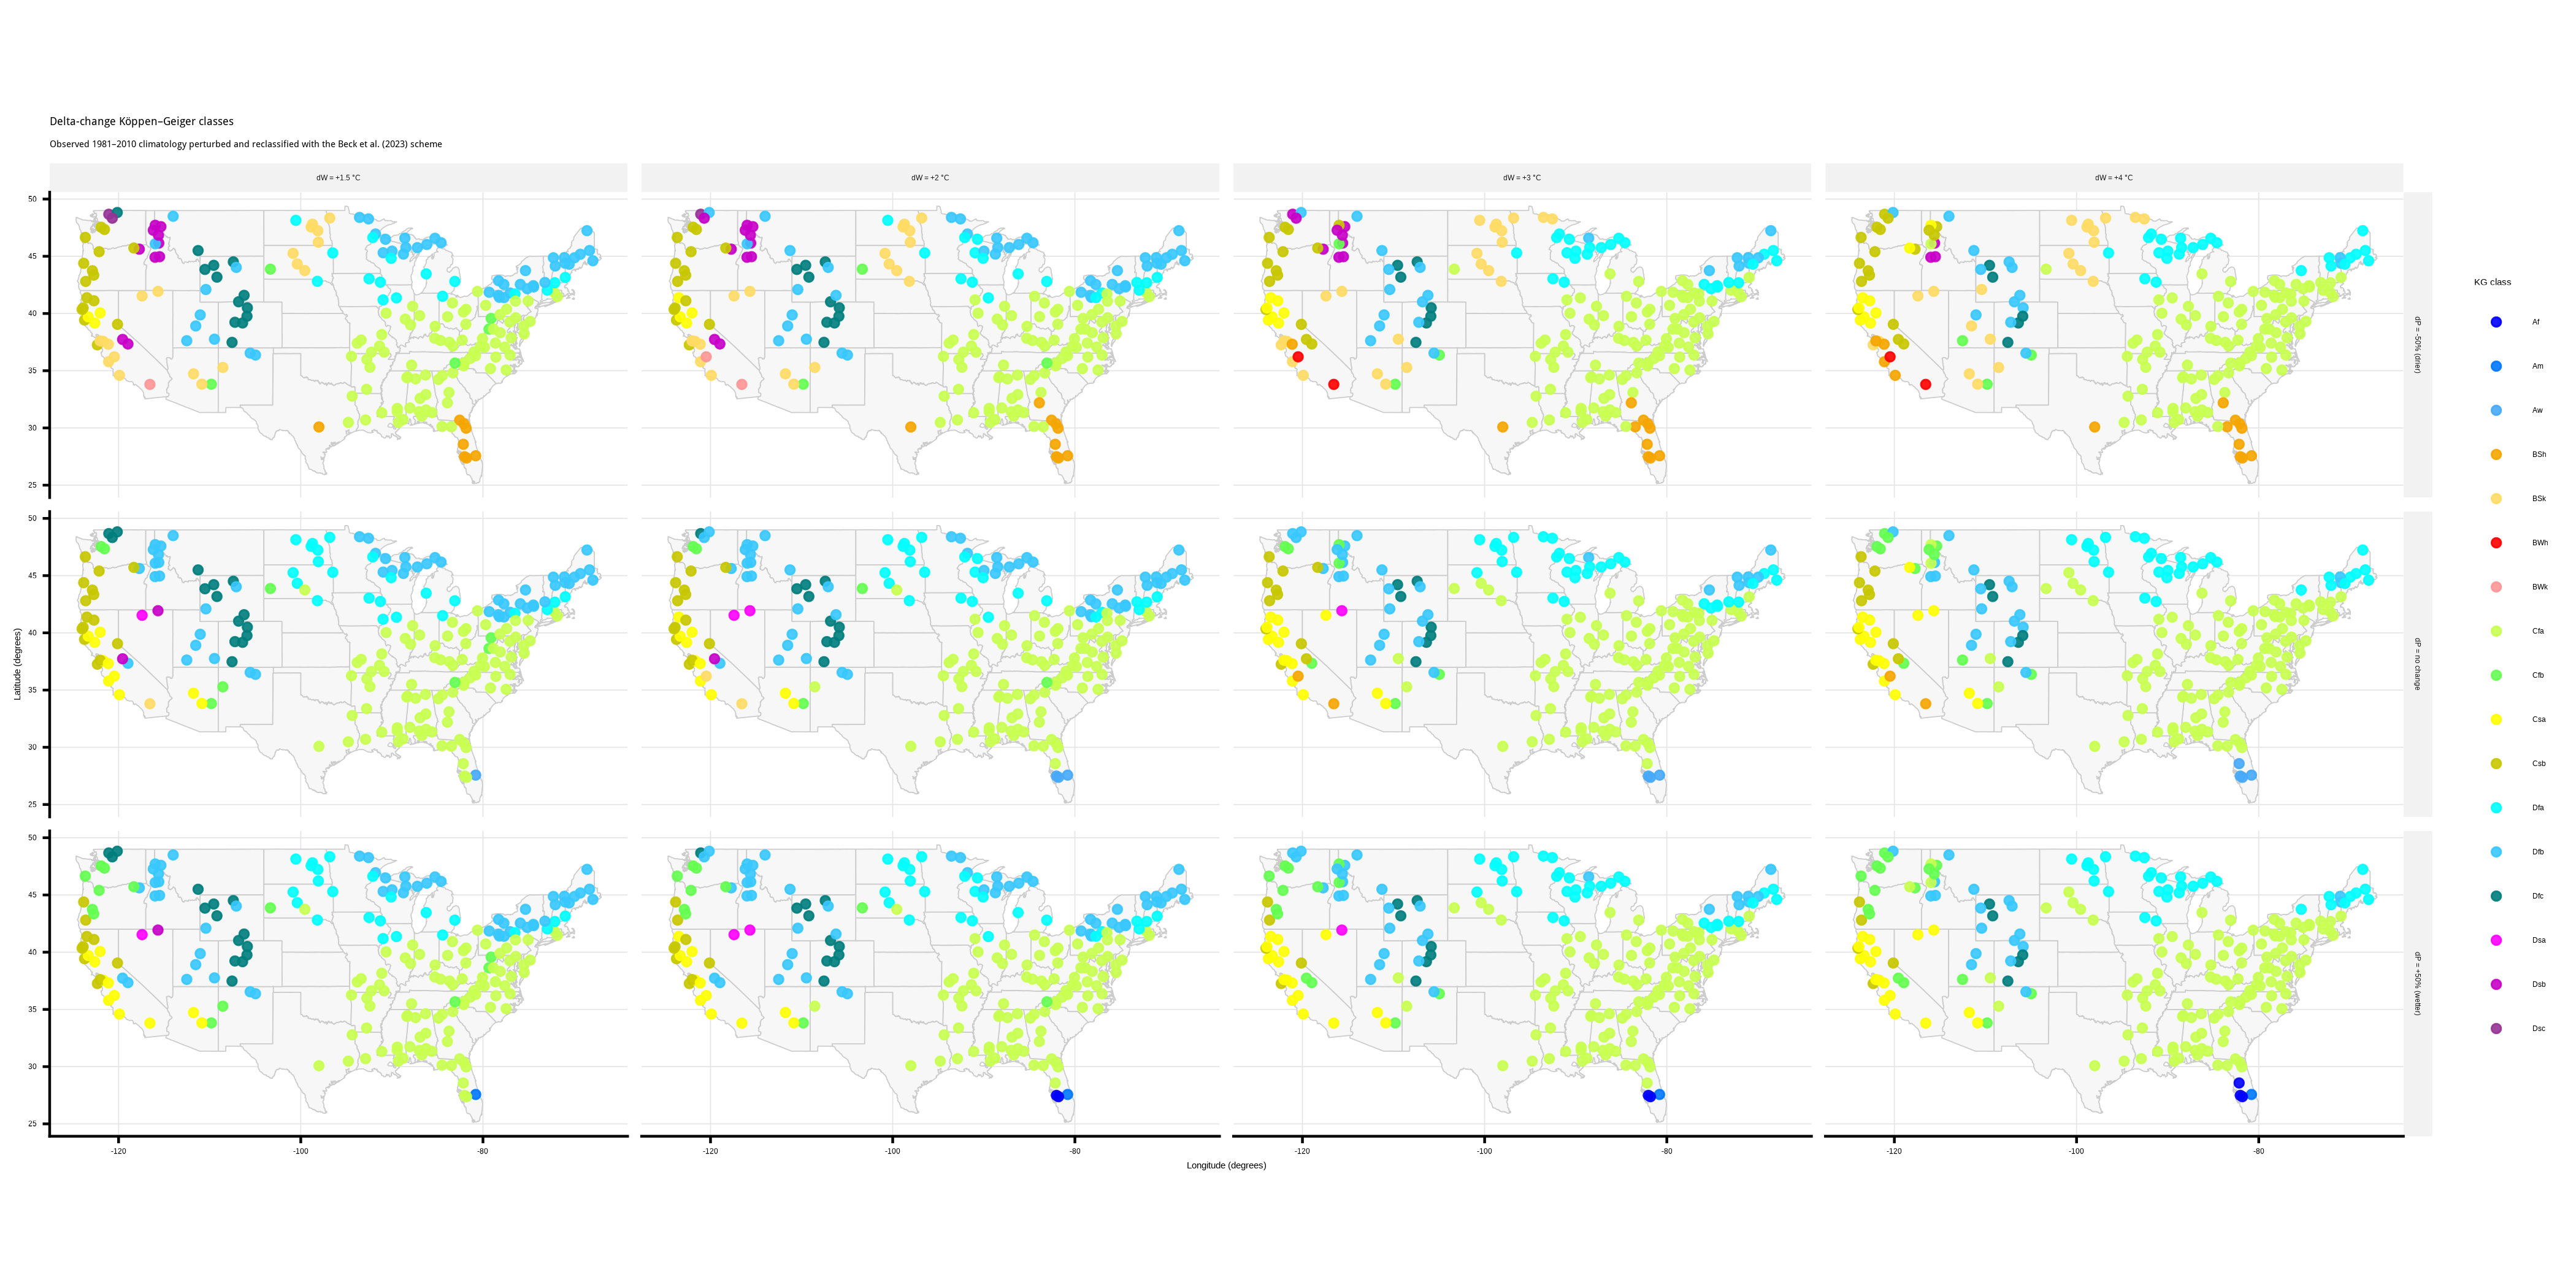
\includegraphics[width=6.27in,height=3.135in,alt={A screen shot of a
chart AI-generated content may be
incorrect.}]{03-writeup/Revision-1/latex/media/media/image8.png}
\caption{Figure 8 Köppen-Geiger classes of the analysed catchments under
delta changes in precipitation of -50\%, 0 and +50\% (rows) and warming
of +1.5, +2, +3 and +4 °C (columns), assigned with the Beck et al.
(2023) scheme applied to perturbed monthly climate normals. Each point
is one catchment, coloured by its future class.}
\end{figure}

For catchment 06614800, Fig. 9 shows how the 121-cell scenario grid
becomes a threshold. The colour of each cell is the fitted probability
that MAR falls in the most vulnerable class (C3) under SPF (left) and
CZIPEF (right), and the white contour marks a probability of 0.5. The
vulnerable region is a wedge that opens towards drier and warmer
conditions: at zero warming the contour lies near a precipitation
multiplier of 0.66 in both panels, and with +8 °C warming it reaches
0.85 under SPF and 1.15 under CZIPEF. Under SPF, 25 of the 121 cells
(21\%) have a probability of at least 0.5, compared with 43 cells (36\%)
under CZIPEF; the extra cells lie at the wetter edge of the wedge, where
warming of 3 °C or more makes C3 the most likely class even with 10-20\%
more precipitation. The threshold summarises this surface: the
precipitation threshold is the multiplier at which the
temperature-averaged probability curve crosses 0.5, which gives 0.67
under SPF and 0.70 under CZIPEF for this catchment, and the CZIPEF
temperature threshold is 3.9 °C.

\begin{figure}
\centering
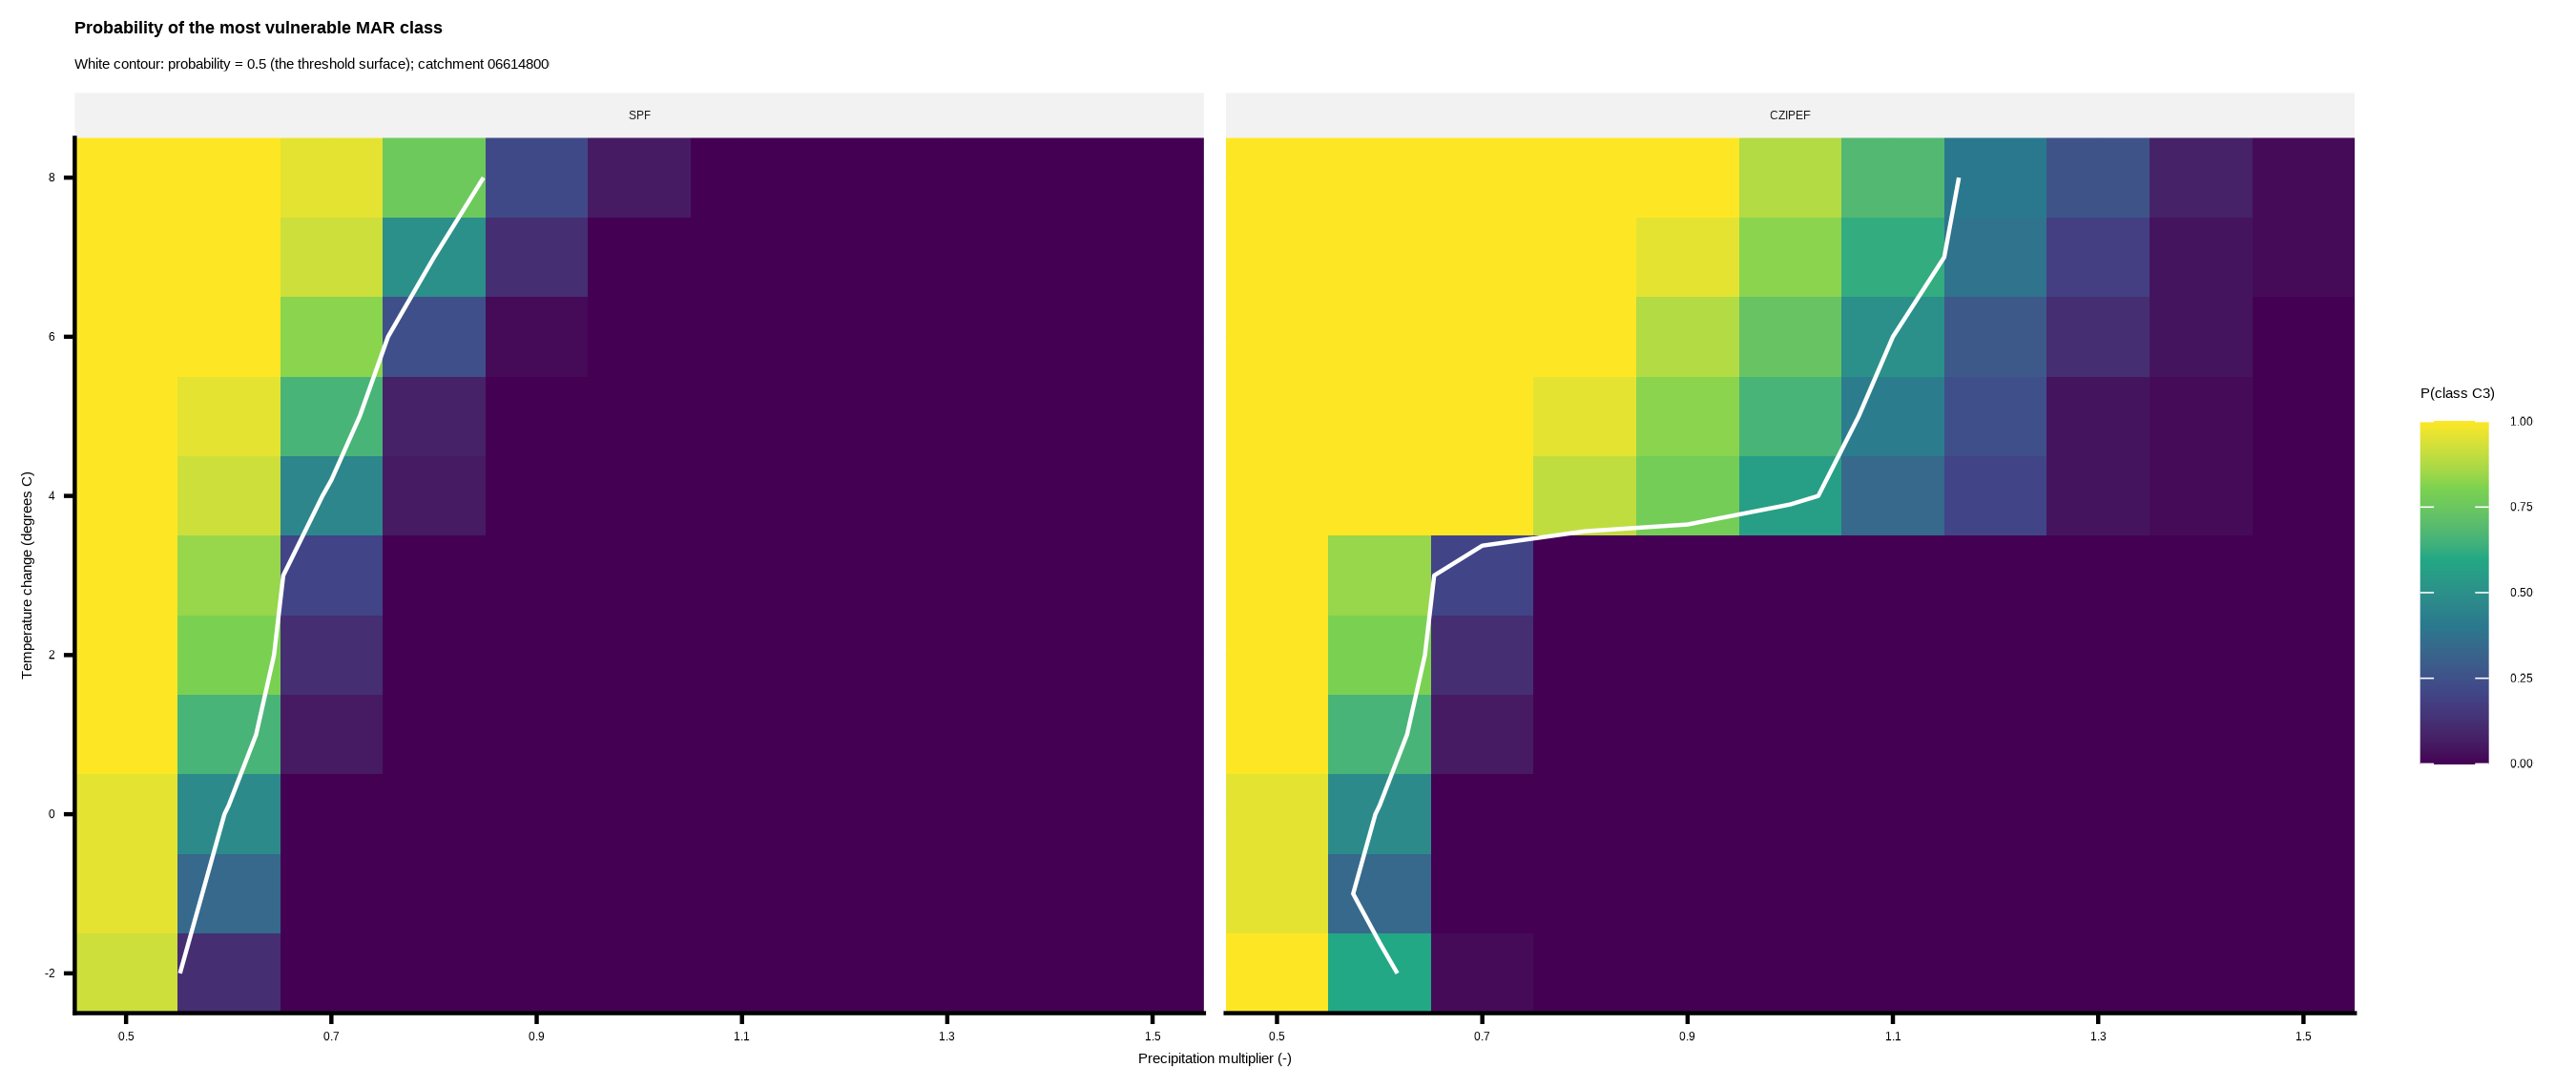
\includegraphics[width=6.26806in,height=2.64651in,alt={A screenshot of a
graph AI-generated content may be
incorrect.}]{03-writeup/Revision-1/latex/media/media/image9.png}
\caption{Figure 9 Probability that MAR is in the most vulnerable class
for catchment 06614800 under SPF (left) and CZIPEF (right). Each cell is
one of the 121 precipitation-temperature combinations, and the white
contour marks a probability of 0.5; the precipitation threshold is where
the temperature-averaged probability curve crosses 0.5.}
\end{figure}

\begin{figure}
\centering
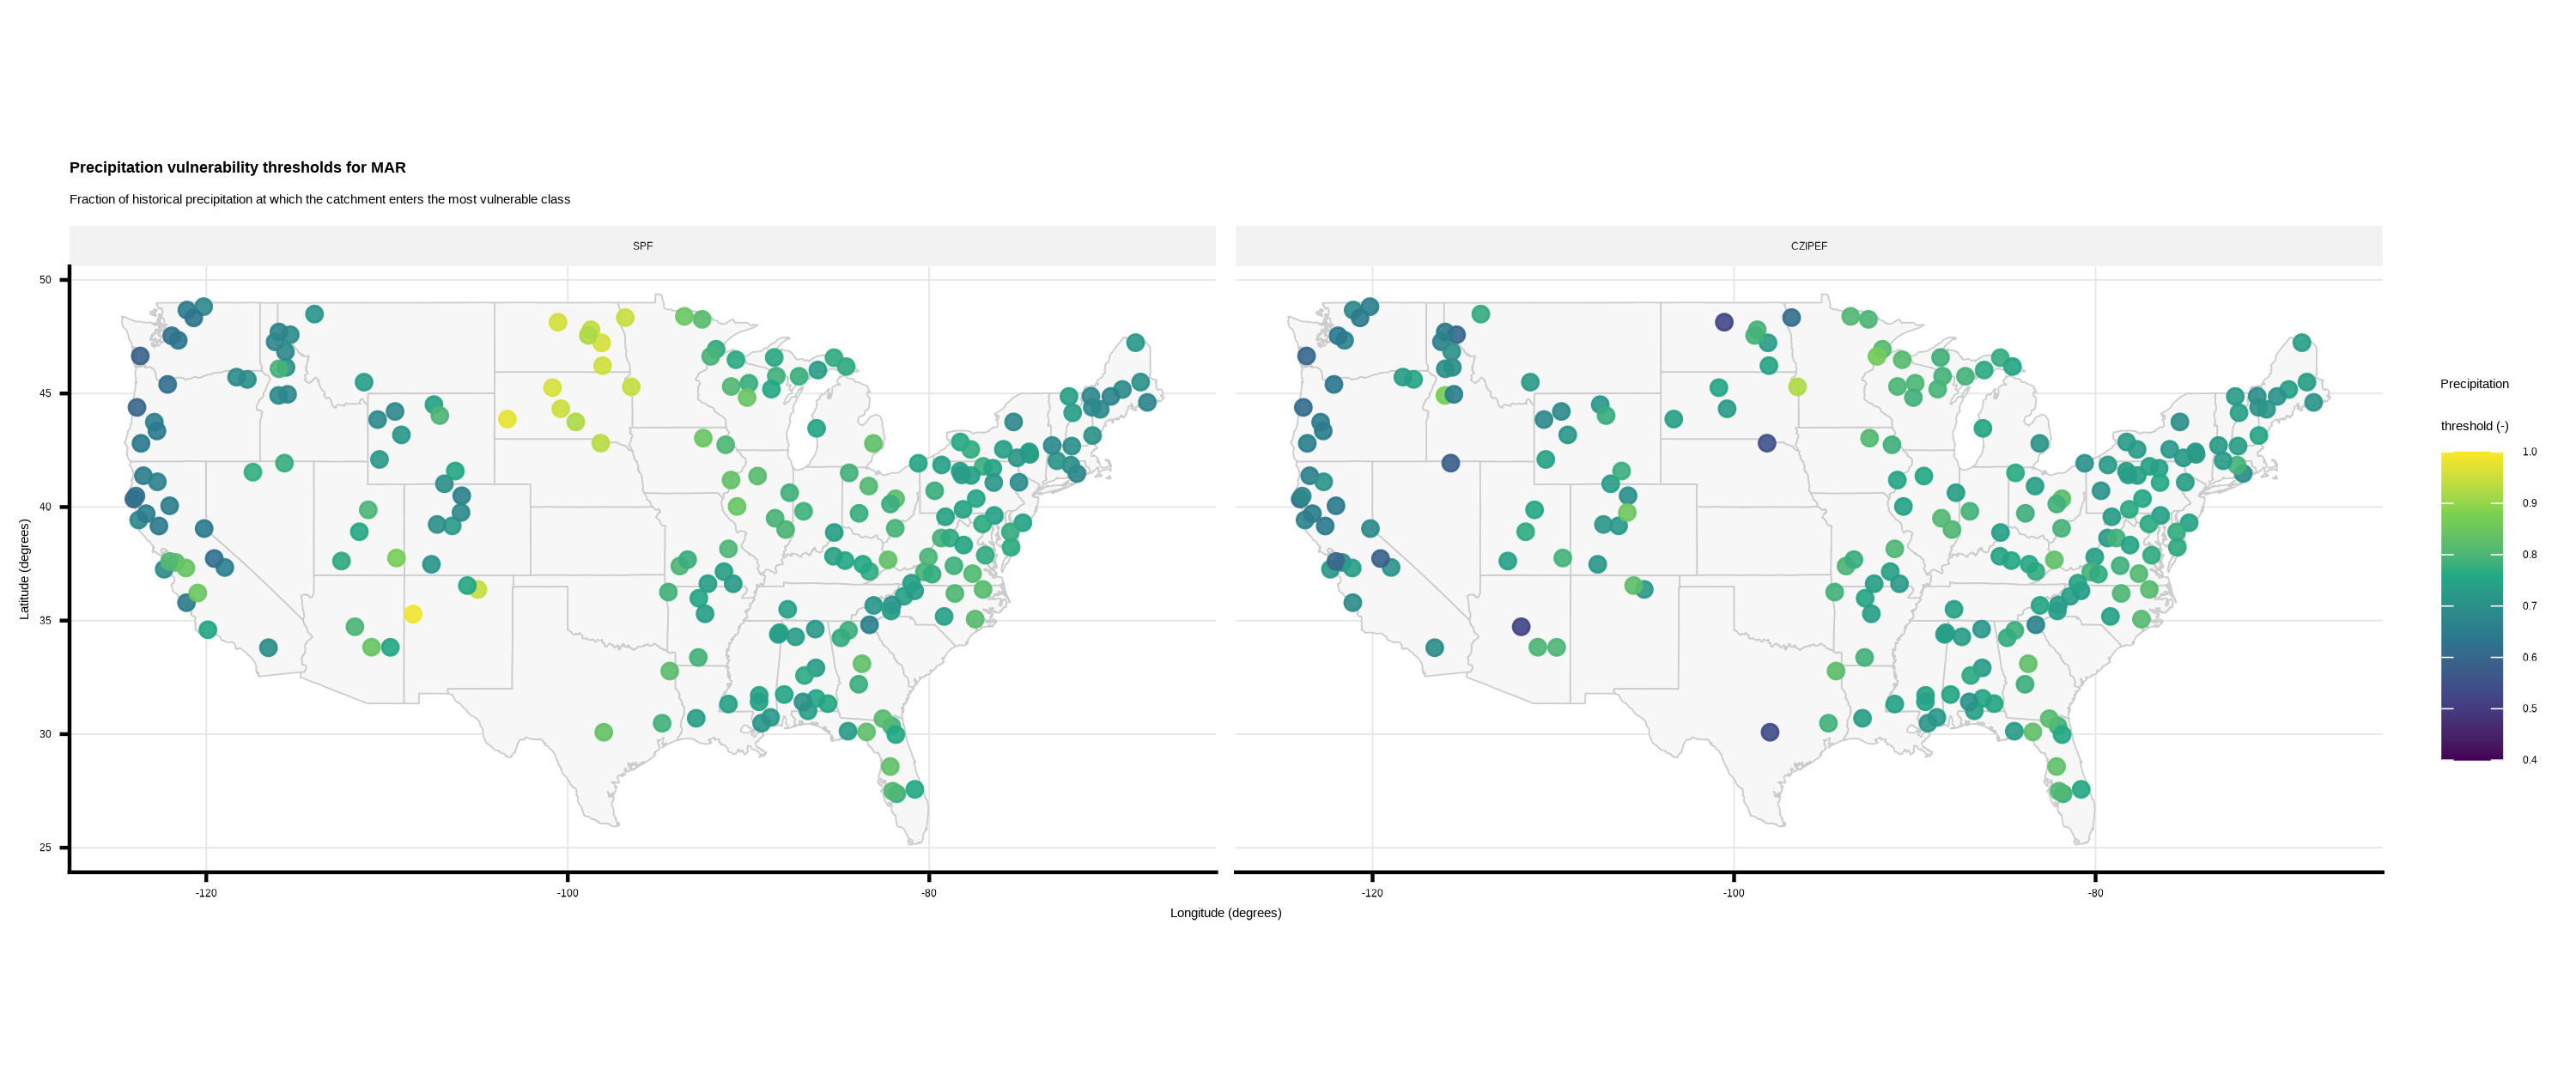
\includegraphics[width=6.26806in,height=2.63258in,alt={A map of the
united states with different colored dots AI-generated content may be
incorrect.}]{03-writeup/Revision-1/latex/media/media/image10.png}
\caption{Figure 10 Precipitation thresholds for MAR under (a) the
stationary parameter framework (SPF) and (b) the climate zone-informed
parameter evolution framework (CZIPEF). Colour gives the threshold, that
is, the fraction of historical precipitation at which the
temperature-averaged probability of the most vulnerable class reaches
0.5. A threshold of 0.8 means that a 20\% reduction in precipitation is
enough, so lower values indicate lower vulnerability.}
\end{figure}

Fig. 10 maps the precipitation threshold for MAR under the two
frameworks, SPF (left) and CZIPEF (right). Each circle is a catchment
and its colour gives the threshold. Across the 222 catchments the
thresholds range from 0.52 to 0.99, with a median of 0.75 and an
interquartile range of 0.71-0.79 under SPF, so a typical catchment
enters the most vulnerable class after a 20-30\% reduction in
precipitation. A threshold of 0.9 or more, where a reduction of only
about 10\% is enough, occurs in 14 catchments under SPF but in only one
under CZIPEF. Both panels share the same broad spatial pattern, as
expected, because both use the same observed climate and the same pools
of behavioural parameter sets; Table 7 gives the thresholds and their
identifiability for all three indicators, and the difference between the
frameworks is examined in Figs. 11 and 12.

The map shows no aridity gradient. Median thresholds are 0.78 in the
wettest quartile of catchments (aridity below 3.6) and 0.77 in the
driest (aridity above 5.7), and across the 217 catchments with a paired
threshold the correlation between threshold and aridity is -0.02 and the
correlation with snow fraction is -0.27. The clearest structure is
climatic rather than geographic: Dfa catchments have a median threshold
of 0.83 and Csa catchments 0.80, whereas Csb catchments of the maritime
Pacific Northwest have a median of 0.65 and Dsc 0.62. The highest
individual thresholds, 0.95-0.99, occur in the northern Great Plains
(the Dakotas, Nebraska and Iowa), where a reduction of only 1-5\% in
precipitation is enough to move MAR into the most vulnerable class, and
the lowest occur on the Pacific coast. Comparing the panels, CZIPEF
raises the threshold in 83 catchments (38\%), lowers it in 74 (34\%) and
leaves it unchanged in 60 (28\%). Neither framework is systematically
more conservative: the median difference is zero and the distribution is
close to symmetric.

The scatter around this pattern shows that baseline aridity alone does
not determine the precipitation threshold. The correlation between the
two is -0.02, and physiographic attributes and the identifiability of
the threshold in the 121-cell grid both contribute, which is why the
threshold is estimated per catchment rather than transferred from an
aridity regression and why the same framework can raise the threshold in
one catchment and lower it in a neighbouring one.

\begin{figure}
\centering
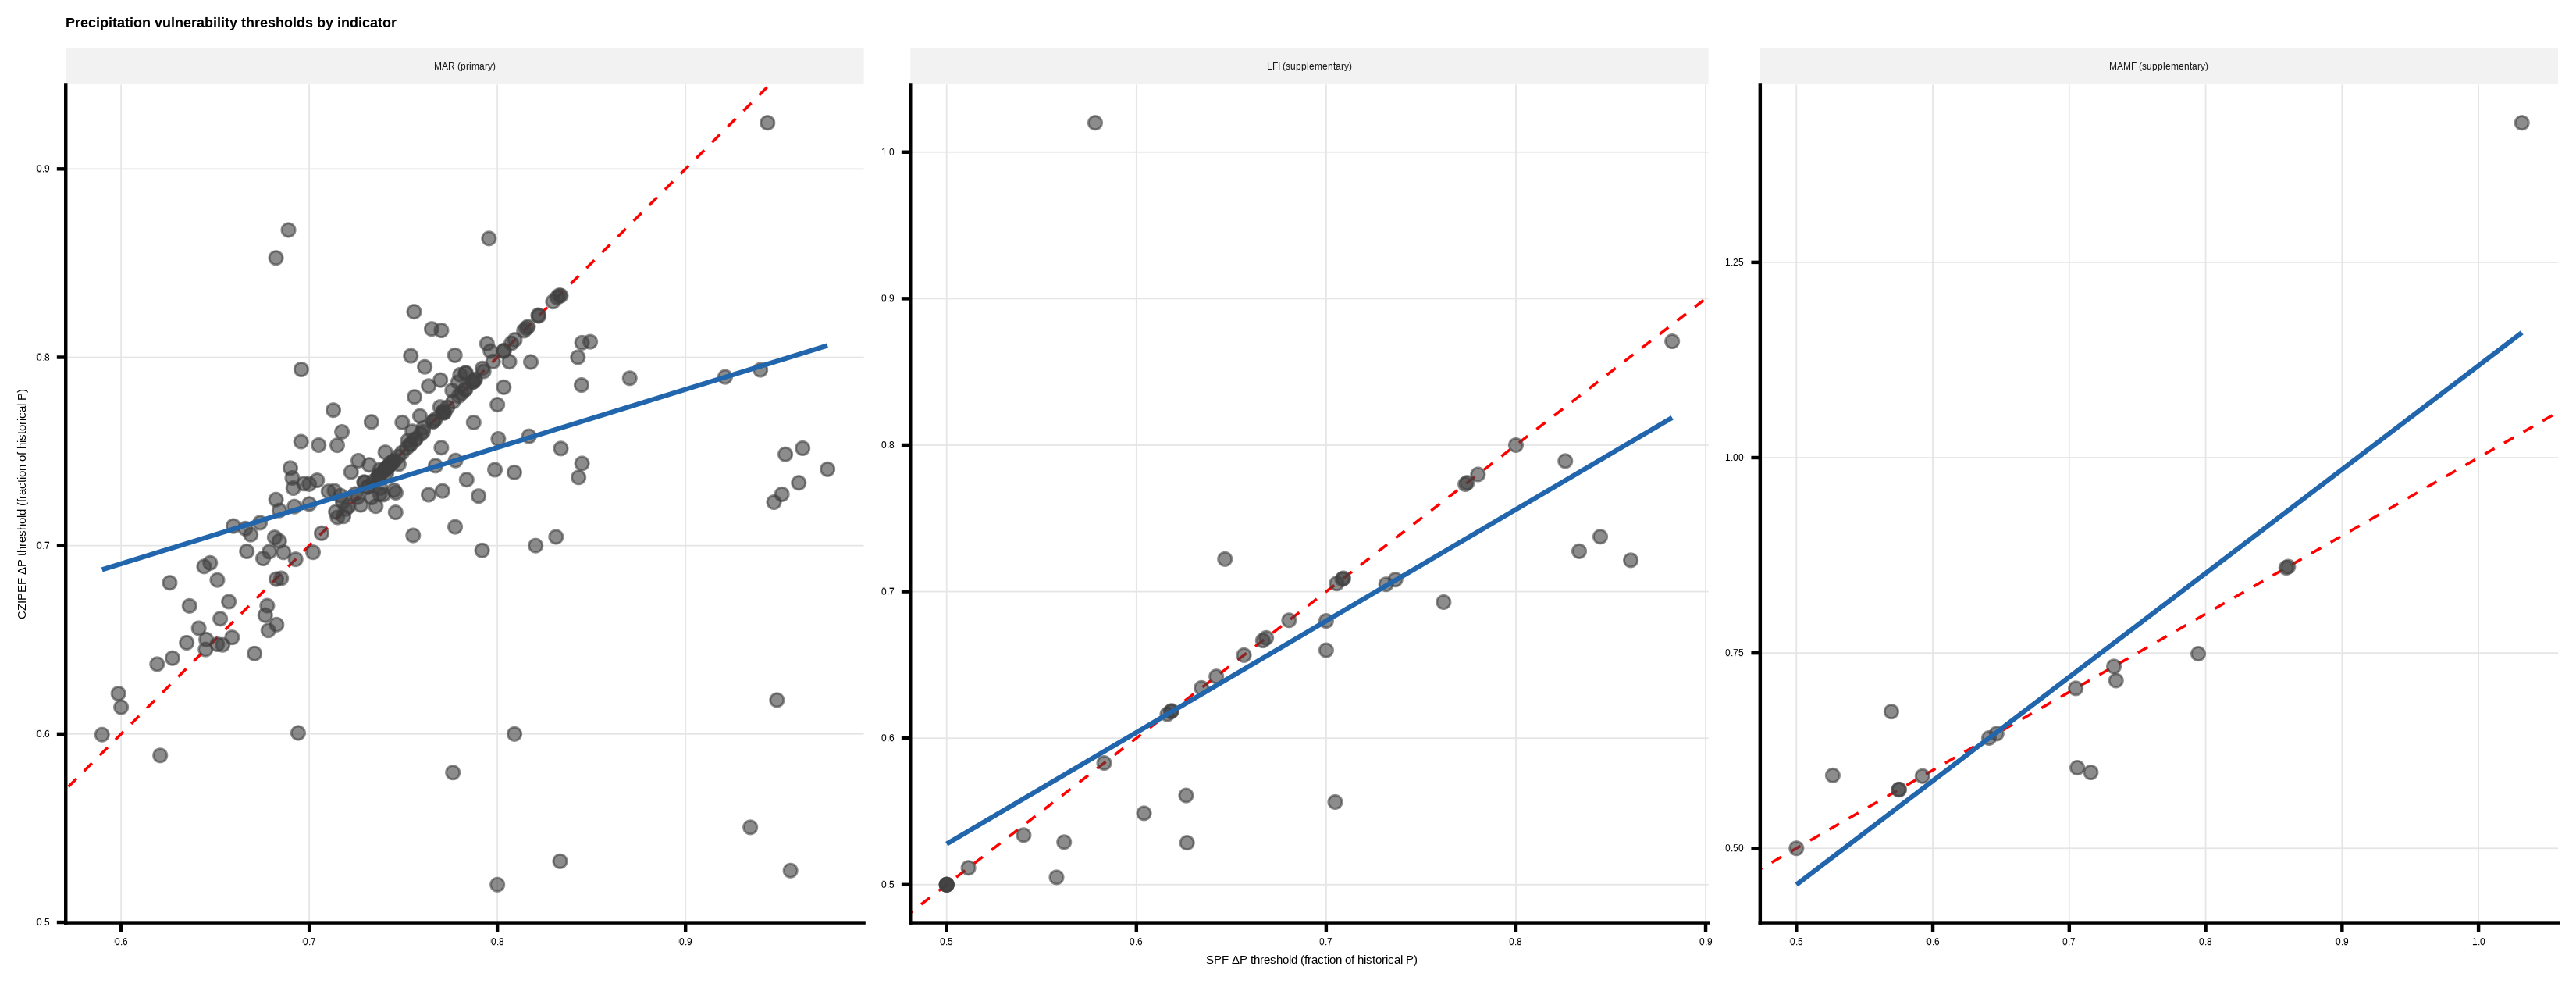
\includegraphics[width=3.86516in,height=1.47579in]{03-writeup/Revision-1/latex/media/media/image11.png}
\caption{Figure 11 SPF against CZIPEF precipitation thresholds for MAR
(n = 217). Grey circles are catchments, the red dotted line is the 1:1
line and the navy dotted line is the ordinary least squares fit (y =
0.505 + 0.309x, R2 = 0.14).}
\end{figure}

The scatter plot in Fig. 11 compares the SPF threshold (x-axis) with the
CZIPEF threshold (y-axis). Each grey point is a catchment, the red
dotted line is the 1:1 reference and the navy dotted line is the
ordinary least squares fit. The regression is y = 0.505 + 0.309x with R2
= 0.14 (n = 217, p \textless{} 0.001), a weak positive association
between the two thresholds. The slope of 0.309 shows that a 0.1 increase
in the SPF threshold corresponds to only about a 0.03 increase in the
CZIPEF threshold, and points lie on both sides of the 1:1 line (38\%
above, 34\% below), so the CZIPEF threshold is not systematically lower
than the SPF threshold. The wide scatter around the regression line
shows that the framework changes individual thresholds substantially
even though the pooled relationship is weak; the low R2 means that the
two thresholds are not interchangeable.

\begin{figure}
\centering
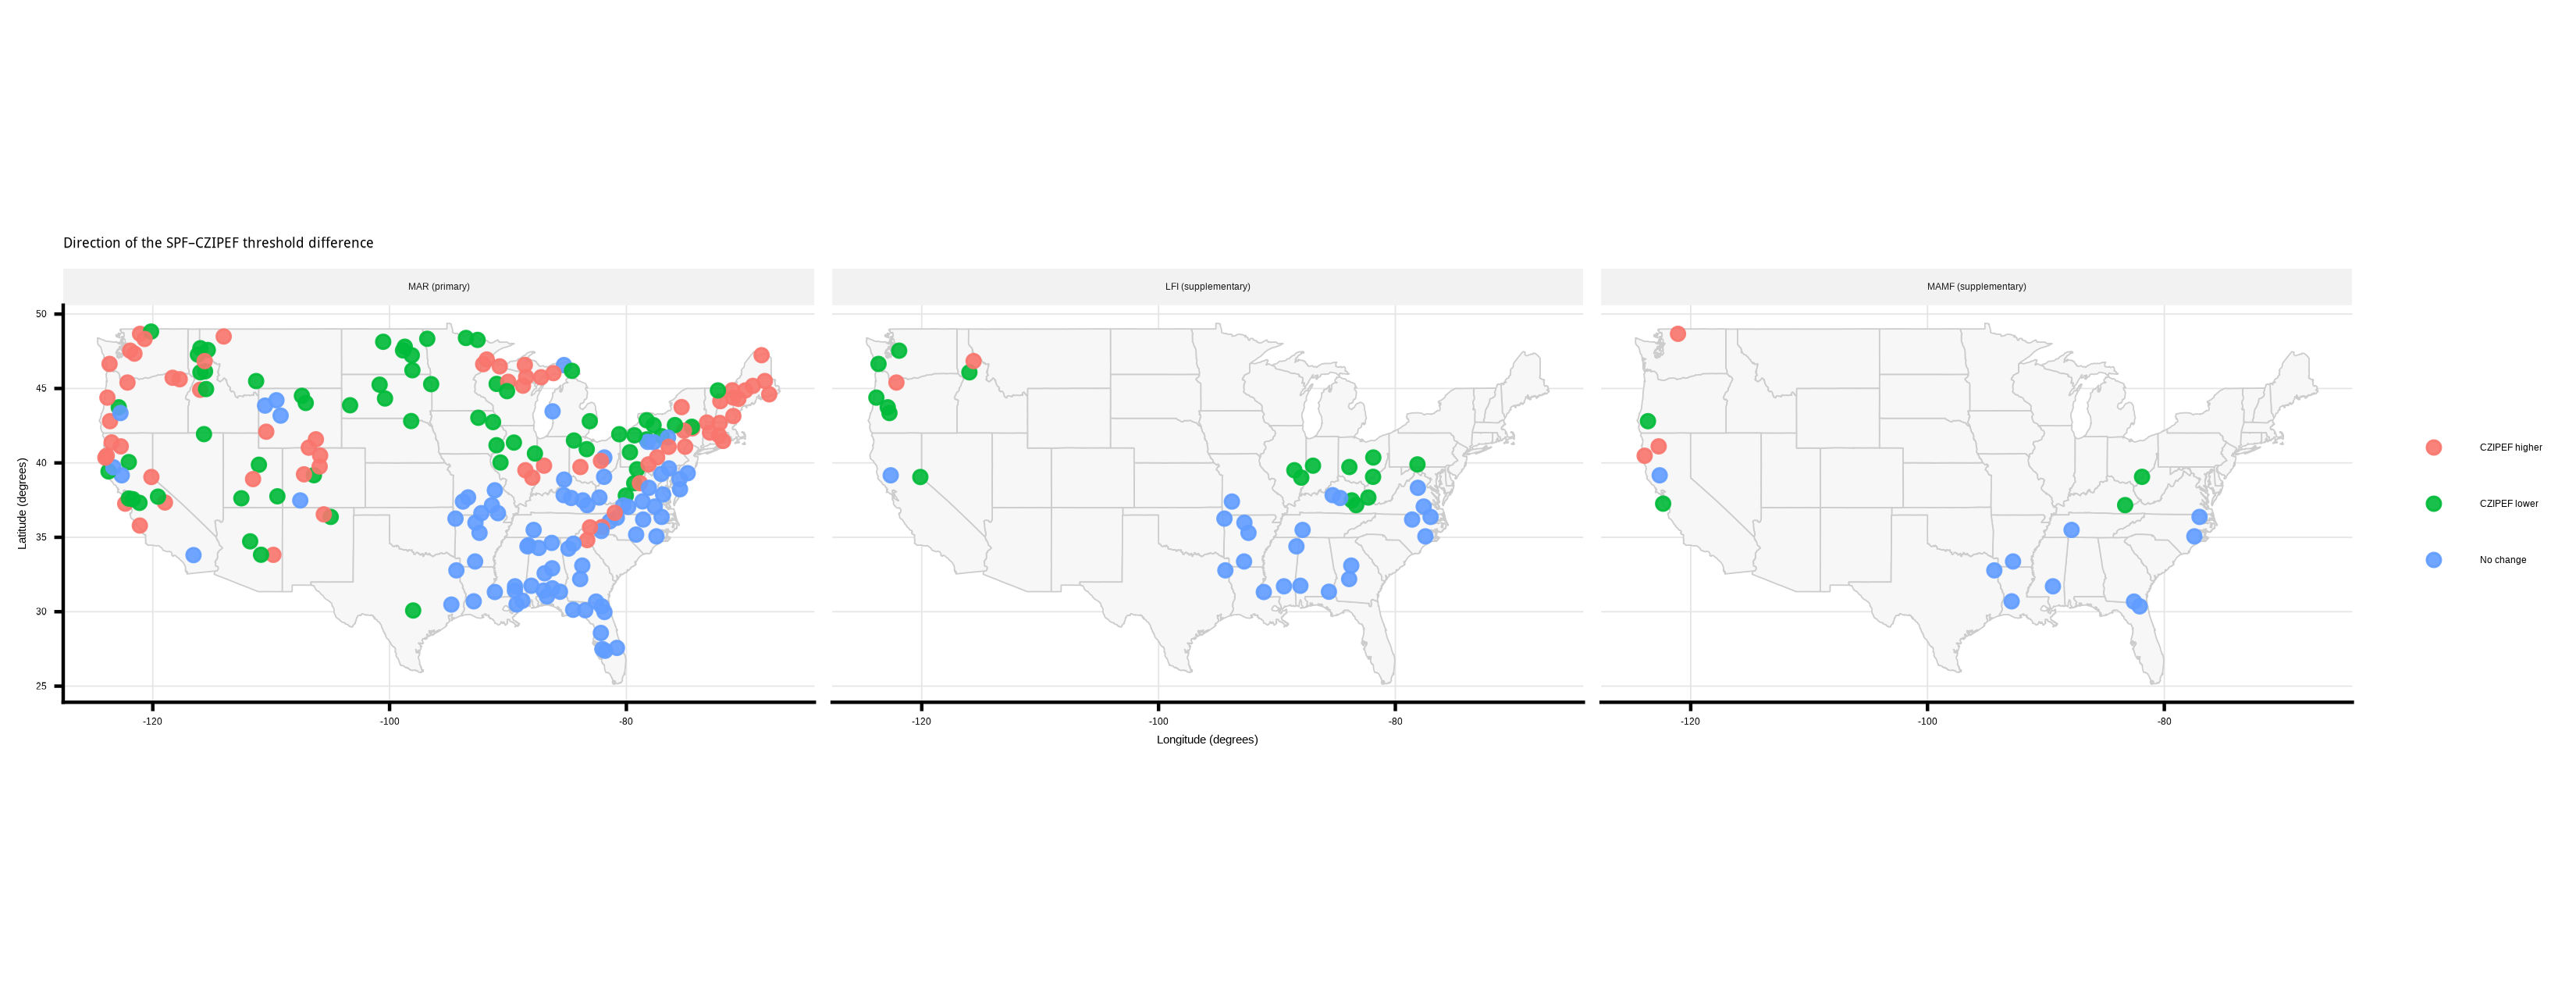
\includegraphics[width=6.13489in,height=2.34241in]{03-writeup/Revision-1/latex/media/media/image12.png}
\caption{Figure 12: Direction of the SPF-CZIPEF difference in the MAR
precipitation threshold. Red circles mark catchments where the CZIPEF
threshold is higher, green where it is lower and blue where the two
thresholds are identical.}
\end{figure}

The difference between the SPF and CZIPEF precipitation thresholds for
MAR is mapped in Fig. 12. Red circles mark catchments where the CZIPEF
threshold is higher (the catchment tolerates less drying before becoming
vulnerable; 83 catchments), green circles where it is lower (74) and
blue circles where the two thresholds are identical (60). The map is
spatially heterogeneous and shows no regional coherence: higher and
lower thresholds occur side by side in the Great Plains, the Midwest and
the west. The paired thresholds are only weakly related overall (slope
0.31, R2 = 0.14) and the median difference is zero, so CZIPEF does not
shift vulnerability in one direction (Table 8). LFI and MAMF have paired
thresholds for only 41 and 17 catchments, so their maps are sparse and
support no regional interpretation.

Fig. 13 shows the cumulative distribution functions (CDFs) of the pooled
behavioural parameter sets for every Köppen-Geiger class with a
parameter pool. Each panel is one HBV parameter and each line is one
class. Twelve classes have a pool, but four of them (BSk, Dsa, Dsc and
ET) contribute 200 sets from a single catchment each, so their curves
are step-like and are shown for completeness rather than interpreted.

\begin{figure}
\centering
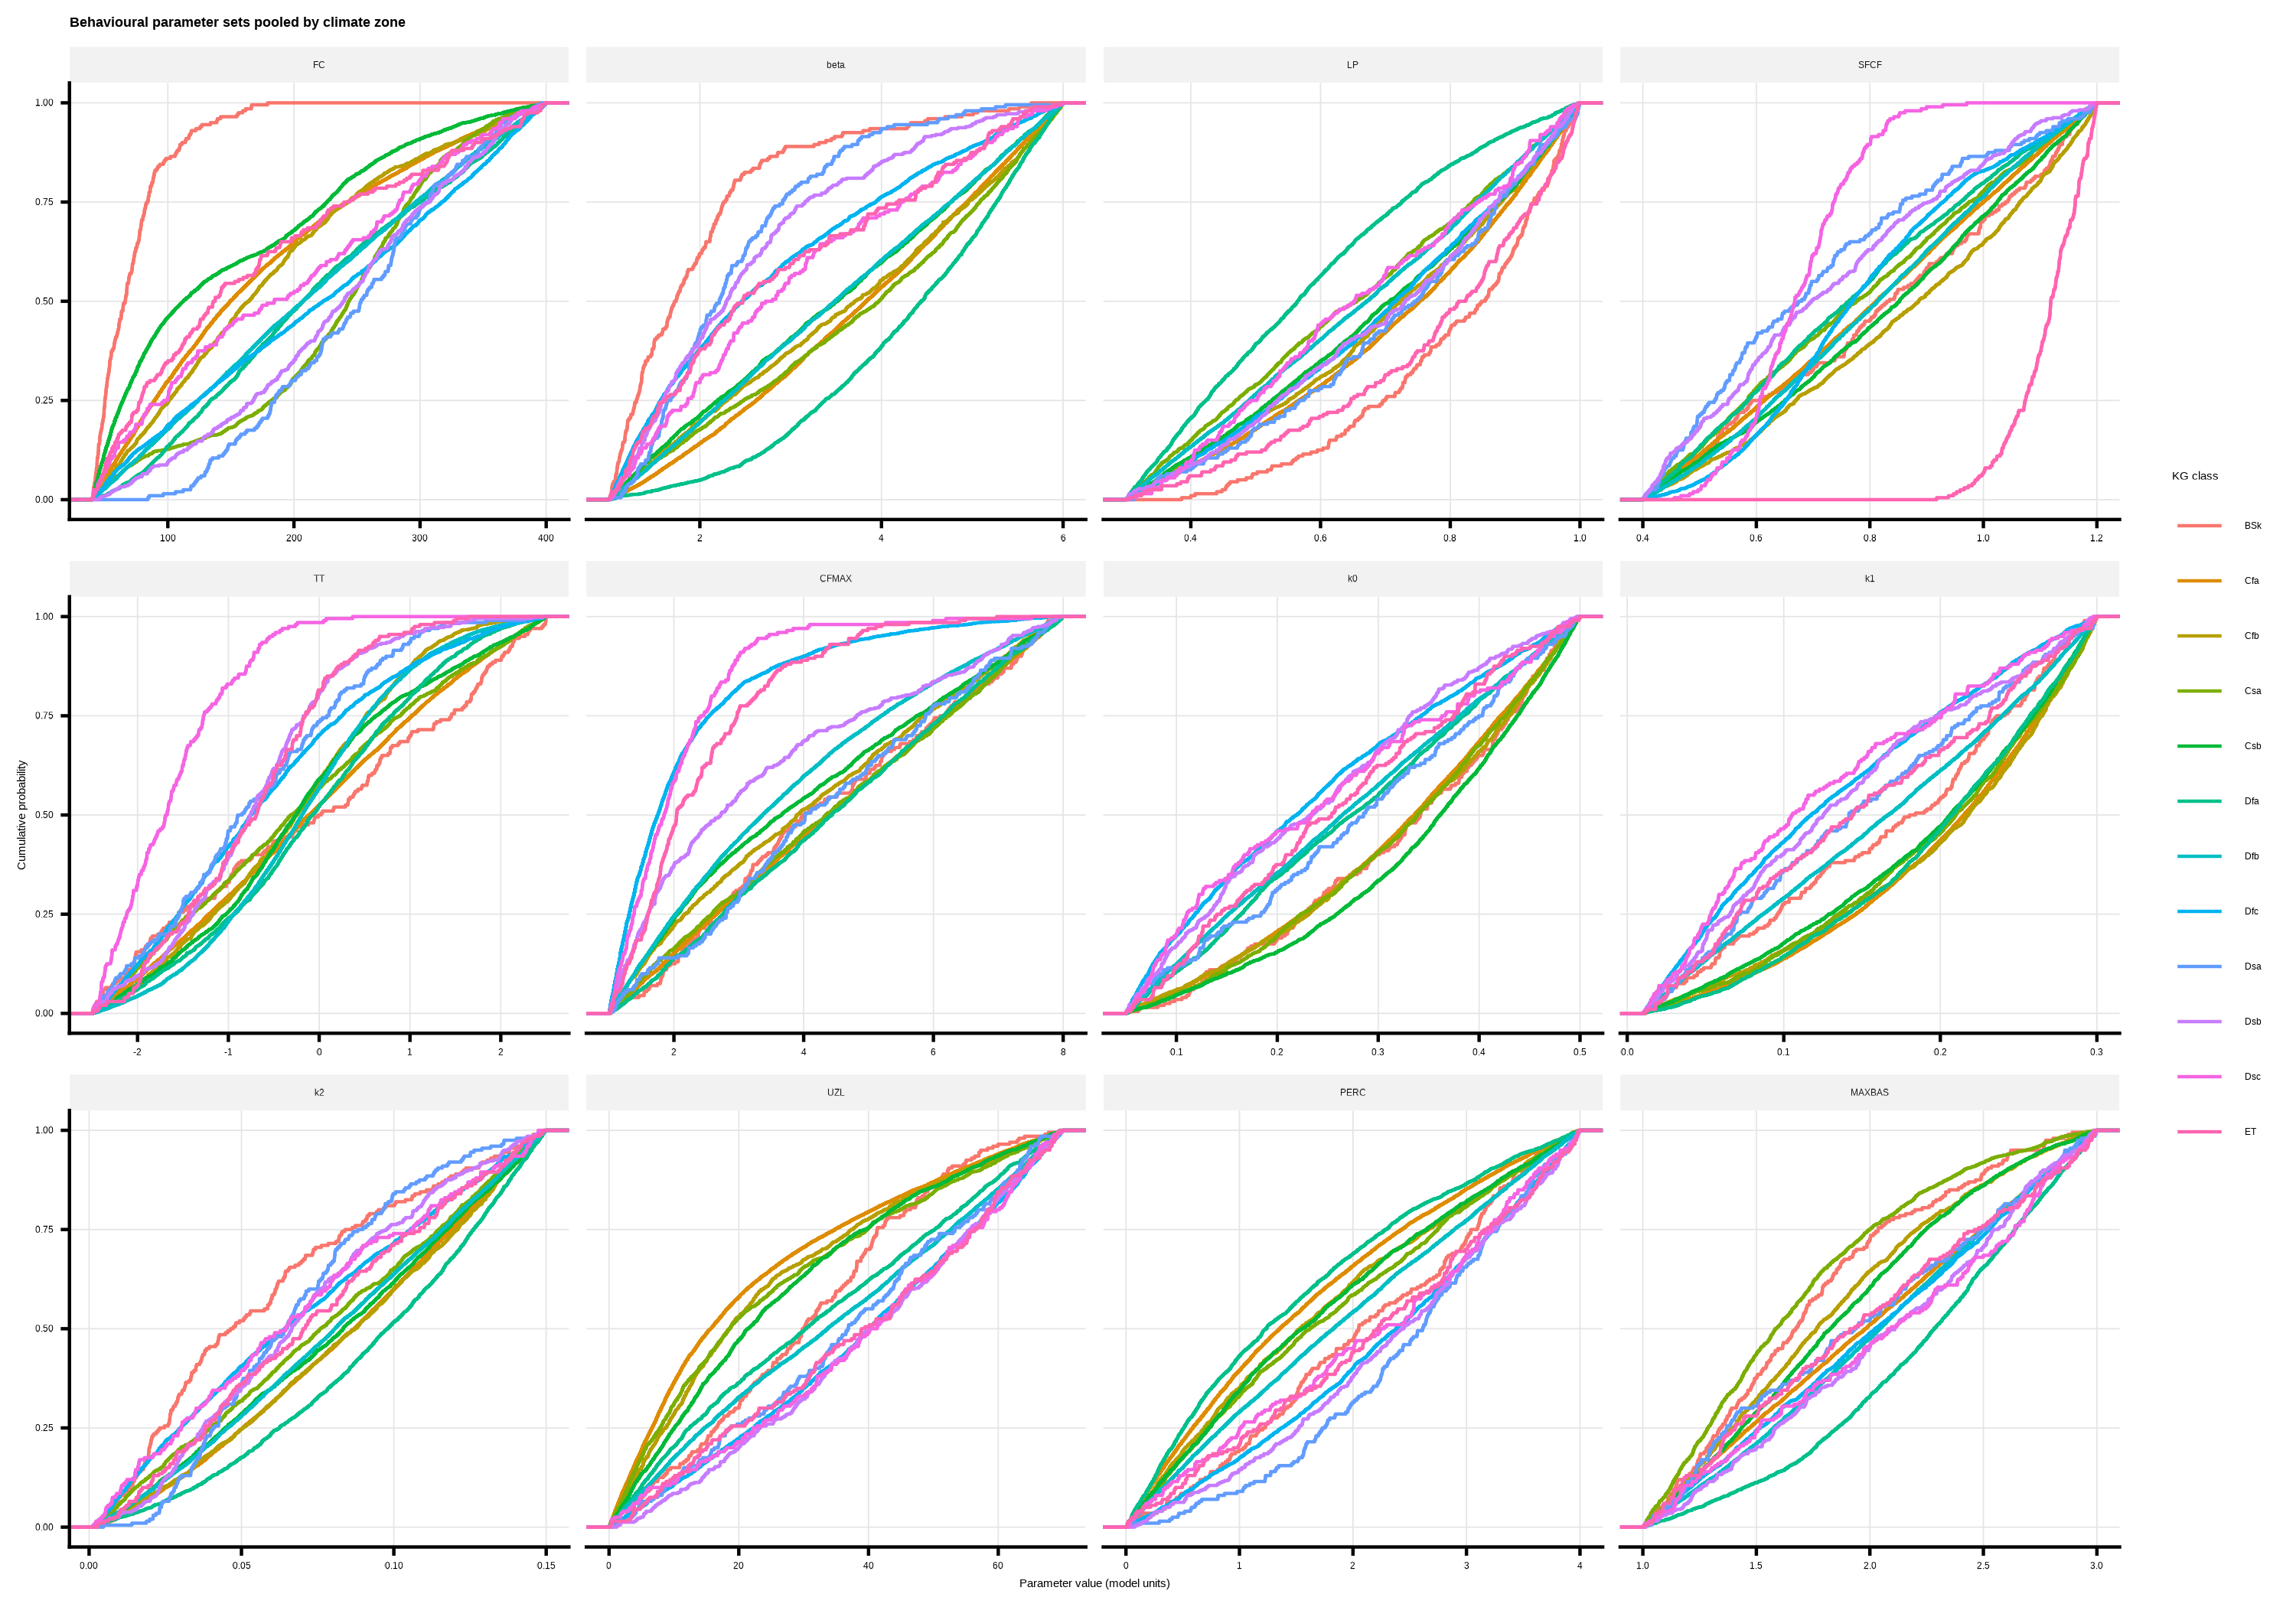
\includegraphics[width=6.26806in,height=4.38764in,alt={A collage of
graphs AI-generated content may be
incorrect.}]{03-writeup/Revision-1/latex/media/media/image13.png}
\caption{Figure 13 Cumulative distribution functions of the pooled
behavioural parameter sets by Köppen-Geiger class. Each panel is one HBV
parameter and each line is one class; classes with a single contributing
catchment are shown as step curves.}
\end{figure}

The CDFs separate by climate zone for all twelve parameters, but the
strength of the separation differs. FC, beta, SFCF, TT and CFMAX
separate most strongly: the median FC of the behavioural sets is 112 mm
in Csb and 150 mm in Cfa, against 207 mm in Dfa, 207 mm in Dfb and 223
mm in Dfc, and the snow parameters shift systematically between the
snow-dominated and the rain-dominated classes (median CFMAX 1.75 mm °C-1
d-1 in Dfc against 4.44 in Dfa). k0, k1, k2, UZL and PERC overlap over
most of their range, so their climate dependence is weak. Every
parameter nevertheless shows some class dependence, which is why the
pools are built by class rather than pooled nationally, and the copula
reproduces each pool without a single out-of-range draw and without
rejecting the marginal distributions in any class (Kolmogorov-Smirnov
test at 5\%).

To separate the climatic from the physiographic control on the parameter
values, each parameter was regressed on climate-zone membership and on
HydroATLAS physiographic attributes, and the variance was partitioned
into climate-only, physiography-only and shared fractions (Table 6, Fig.
S6). Climate explains the largest share for CFMAX (63\%), k1 (45\%),
PERC (34\%), k0 (34\%) and UZL (32\%) and the smallest for MAXBAS (6\%),
SFCF (11\%) and TT (15\%). Physiography explains more than climate for
beta (39\% against 29\%), k0 (47\% against 34\%), PERC (48\% against
34\%), UZL (53\% against 32\%) and MAXBAS (31\% against 6\%). Adding
climate-zone membership to a physiography-only model raises the
explained variance by 0.03-0.09 for beta, LP, TT, k2 and PERC but by
only 0.03 for MAXBAS and CFMAX, and a random forest on the same
attributes (Fig. S7) ranks mean precipitation, snow fraction and
available water storage highest for FC, consistent with the variance
partitioning. Parameter values are therefore jointly controlled by
climate and physiography, and the climate-zone pools capture only part
of the between-catchment variation. This is a limit of the framework,
not a property of the model.

\begin{figure}
\centering
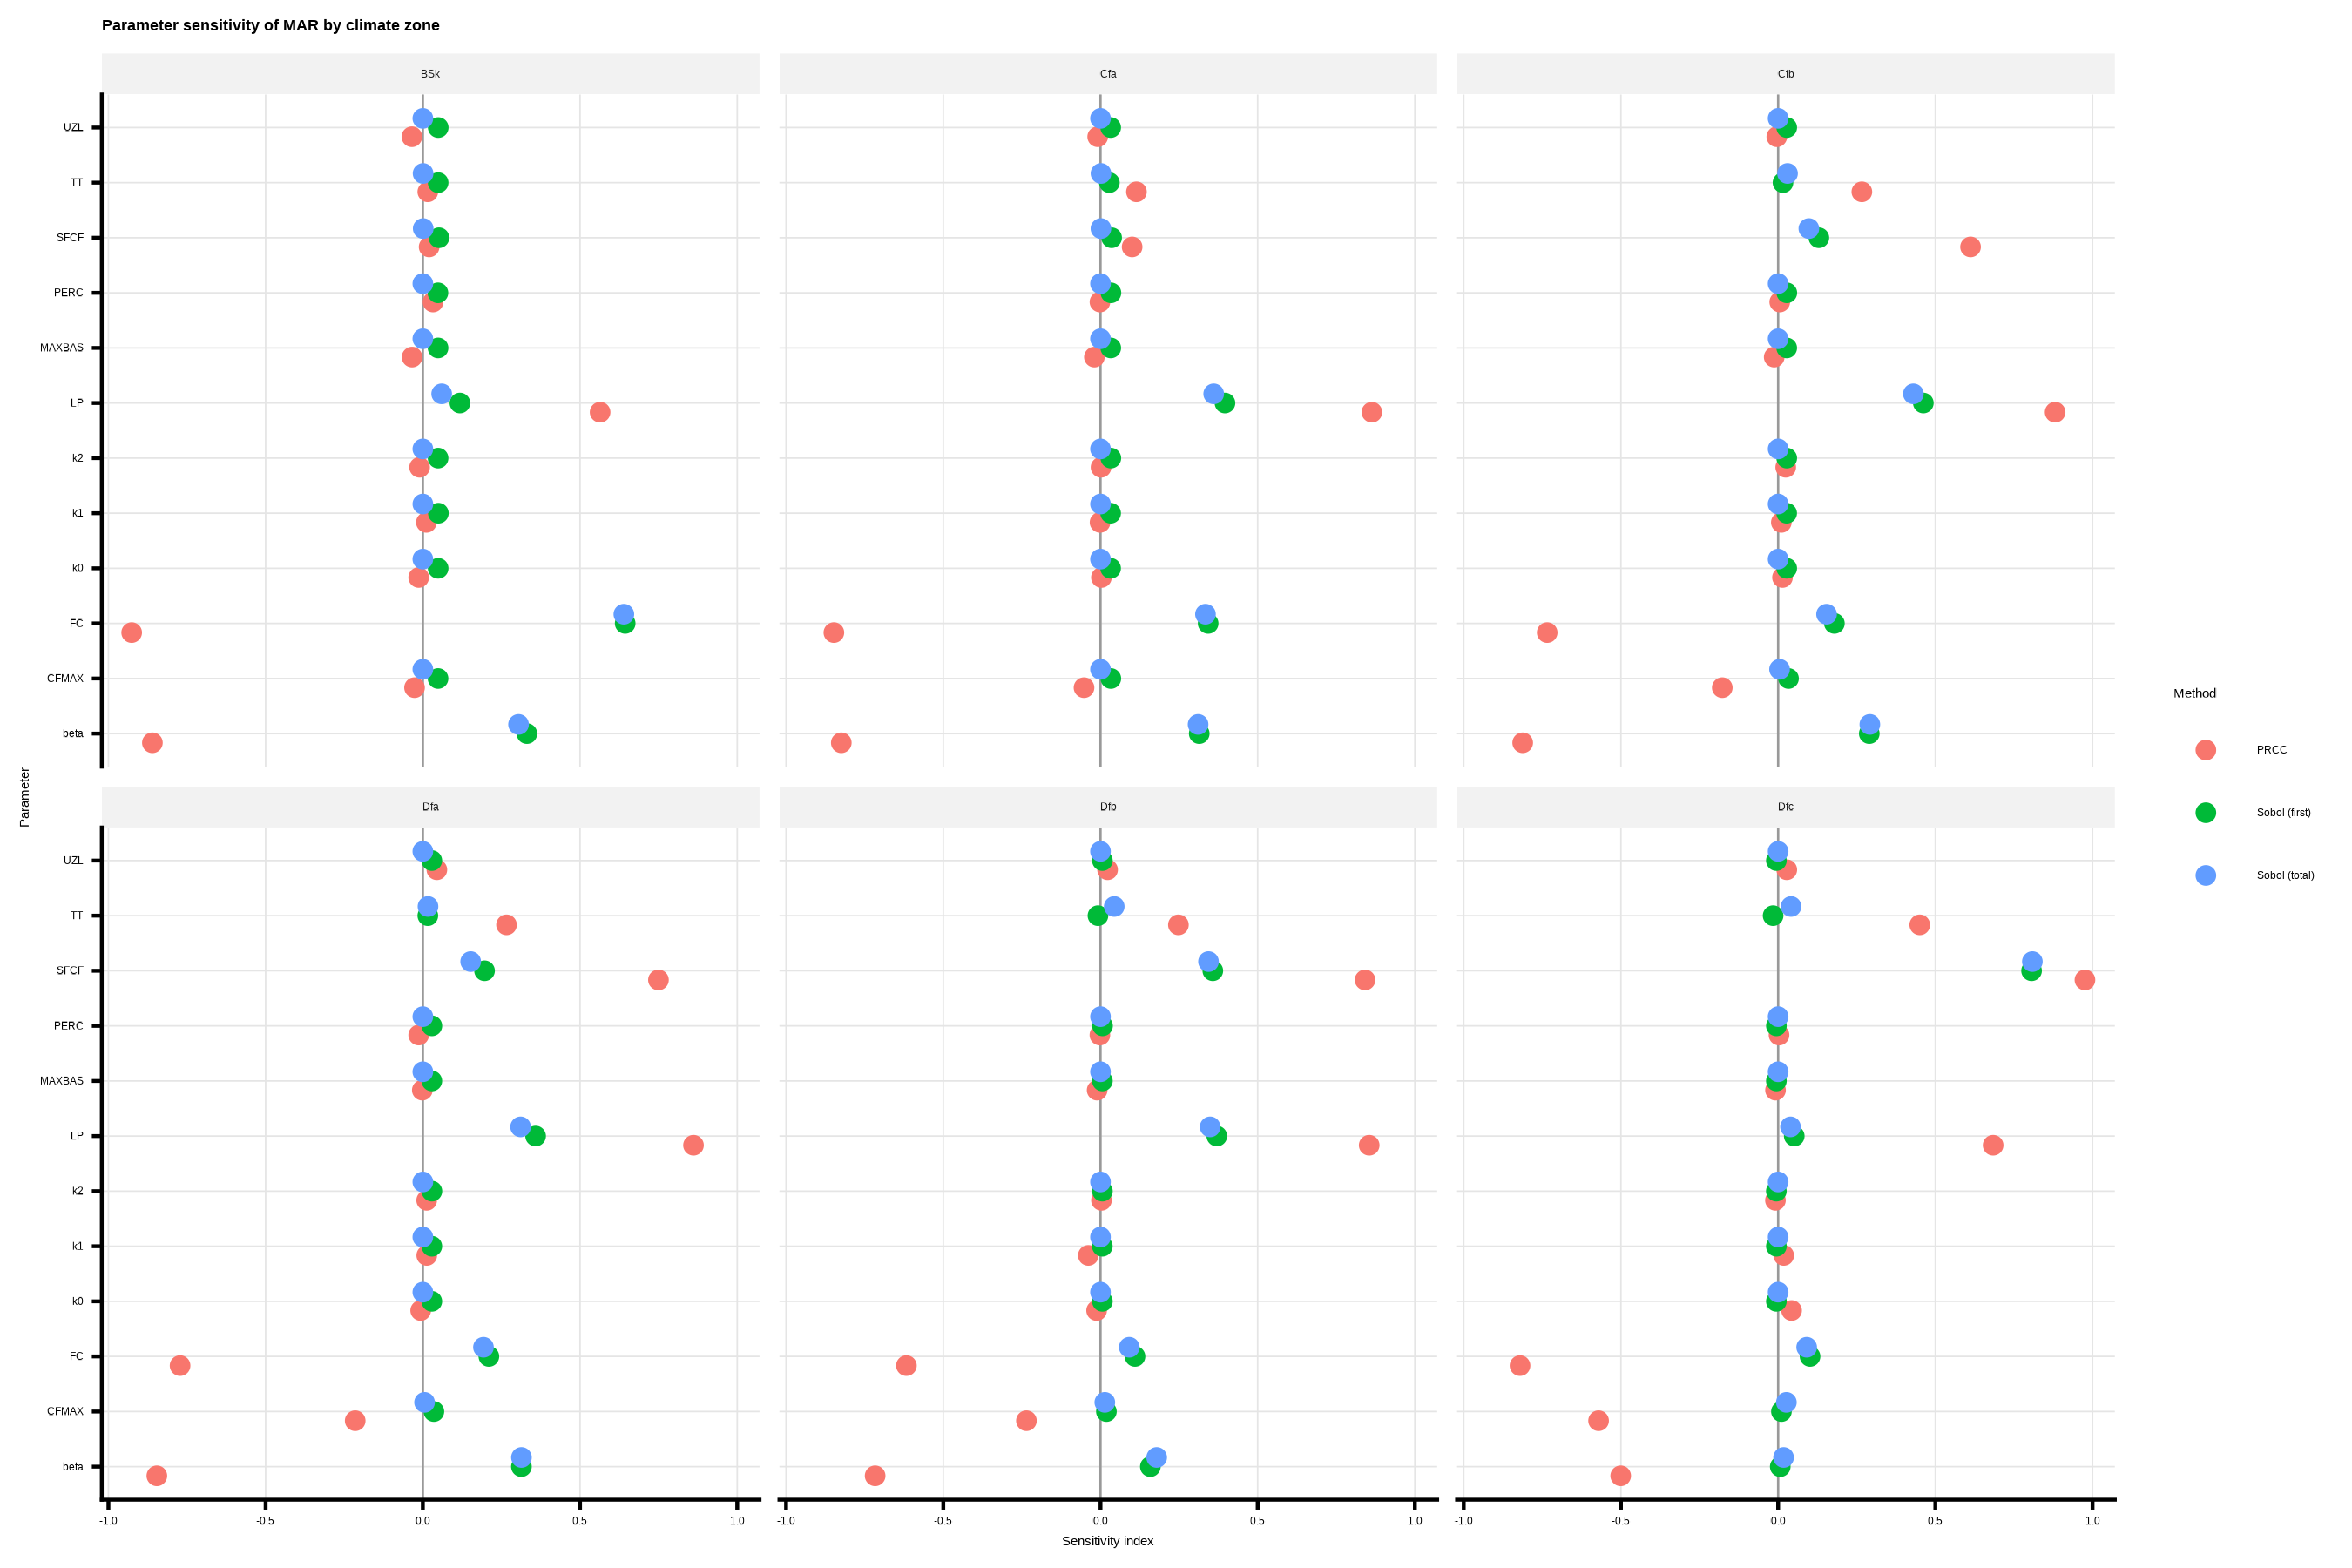
\includegraphics[width=6.26806in,height=4.1787in]{03-writeup/Revision-1/latex/media/media/image14.png}
\caption{Figure 14 PRCC and Sobol sensitivity of the HBV parameters for
MAR in six catchments representing the six dominant classes (BSk, Cfa,
Cfb, Dfa, Dfb and Dfc).}
\end{figure}

Parameter sensitivity is quantified with two global methods: partial
rank correlation coefficients (PRCC) between each parameter and each
indicator, and variance-based Sobol indices, both computed for six
catchments, one in each of the six dominant classes (BSk, Cfa, Cfb, Dfa,
Dfb and Dfc). PRCC uses 2000 Latin-hypercube draws per catchment and
Sobol uses a 512-sample base matrix (13,312 model runs). Sensitivity is
computed for the three vulnerability indicators, MAR, LFI and MAMF. Fig.
14 shows MAR; Fig. S8 shows LFI and MAMF, and Table 9 summarises which
parameters are significant in each class and indicator.

For MAR, beta, FC and LP are significant in every class, and CFMAX, SFCF
and TT join them in Cfb, Dfa, Dfb and Dfc (Table 9). The Sobol indices
agree with the PRCC ranking: for the BSk catchment the first-order
indices are 0.64 for FC, 0.33 for beta and 0.12 for LP, while the
remaining nine parameters have total indices below 0.002. For LFI, beta,
FC, LP, k1 and k2 recur across classes, with TT, CFMAX and SFCF entering
where snow is important. MAMF is the most parameter-rich indicator:
eight to ten parameters are significant in Cfb, Dfa, Dfb and Dfc, and
MAXBAS is significant only in Cfa, where routing has a stronger
influence on high flows. The sign of the FC effect differs between
indicators: the PRCC of FC is -0.93 to -0.62 for MAR and -0.45 to -0.06
for MAMF but -0.03 to +0.43 for LFI, so more storage lowers total runoff
and flood peaks while sustaining low flows. Six catchments cannot
represent all 222, so Table 9 is a class-level summary rather than a
catchment-level map.

The parametric uncertainty of the three indicators differs by an order
of magnitude and explains the identifiability results. Across the 200
retained behavioural sets the coefficient of variation of the ensemble
is 5-11\% for MAR, 16-142\% for MAMF and 50-228\% for LFI (Fig. S9). MAR
is therefore tightly constrained by the calibration, whereas LFI and
MAMF depend strongly on the parameter set and their thresholds cross 0.5
in far fewer catchments, which is why the supplementary indicators are
reported as supporting evidence rather than as the basis of the main
conclusion.

\section{5. Discussion}\label{discussion}

The findings discussed here offer insights into computational hydrology,
particularly by addressing the ongoing challenges of reconciling
parameter non-stationarity with climate regime changes caused in
physical processes. While focusing on the current literature that
progressively recognizes the limitations of standard hydrological
modeling paradigms under changing climatic conditions, this study
intends to contribute constructively by integrating climate
categorization frameworks with parameter dynamics. The discussion that
follows reviews on the implications of this integration, explores
methodological considerations, investigates parameter sensitivities
across climates, examines spatial vulnerability patterns, and outlines
potential impacts for water resources management and future research
directions.

\subsection{5.1 Paradigm Shift from Stationarity to Climate-Informed
Non-Stationarity and Physical Process
Understanding}\label{paradigm-shift-from-stationarity-to-climate-informed-non-stationarity-and-physical-process-understanding}

The conventional stationarity assumption in hydrological modeling, once
considered to be the foundation of water resources planning, has been
increasingly recognized as inappropriate under present climate
conditions (Milly et al., 2008; Razavi et al., 2015). The offered
Köppen-Geiger-based non-stationarity framework presented is a
substantial methodological improvement over standard techniques by
offering physically grounded constraints for parameter evolution rather
than depending on merely statistical alterations. The precipitation
threshold differs between SPF and CZIPEF in 157 of the 217 catchments
with a paired threshold (72\%), being higher under CZIPEF in 83 and
lower in 74, while 60 catchments have an identical threshold. The
framework therefore changes the estimated vulnerability of most
catchments, but not in a consistent direction. This observation, to a
modest extent, corresponds with non-stationary frequency analysis, where
Garcia-Aristizabal et al. (2015) determined that integrating climate
covariates in extreme value distributions considerably improves model
performance and reduces projection uncertainty.

The regression equation y = 0.505 + 0.309x, R2 = 0.138 between SPF and
CZIPEF precipitation thresholds shows that climate-zone-based resampling
changes individual vulnerability estimates substantially, although the
pooled relationship is weak and its direction is not systematic. The
size of these adjustments shows that a stationarity-based threshold can
under- or overstate adaptability by a substantial margin even when the
average change is near zero, a concern highlighted by recent work in
non-stationary hydro-climatology (Brunner \& Gilleland, 2020; Slater et
al., 2021). The theoretical foundation for these threshold changes
arises from the Köppen-Geiger system\textquotesingle s explicit
integration of temperature-precipitation regime features that regulate
hydrological process dynamics. Unlike purely temporal trend-based
approaches to non-stationarity (Vogel et al., 2011), our framework
preserves process interpretability while accommodating parameter
evolution, addressing a critical limitation identified in recent reviews
of non-stationary hydrological modeling (Serinaldi \& Kilsby, 2015).

CZIPEF~presents an analytical foundation for understanding parameter
evolution under fluctuating climatic regimes. The examination of
behavioural parameter distributions across climate zones shows that FC,
beta, CFMAX, SFCF and TT separate most strongly between zones, while k0,
k1, k2, UZL and PERC separate least; the variance partitioning in Table
6 shows that this separation is only partly climatic, because
physiography explains more of the variation in beta, k0, PERC and UZL.
This parameter-climate relationship pattern offers significant insights
into the physical processes controlling catchment response. The
separation of FC between classes reflects differences in soil-atmosphere
relationships across climate regimes, with arid systems typically
presenting lower soil moisture storage capacity because of higher
evapotranspiration rates and different soil development processes,
although part of the signal is physiographic (Melsen et al., 2018). The
snow-related metrics (CFMAX, SFCF, TT) demonstrating significant climate
sensitivity logically correspond to the fundamental energy balance
differences between snow-dominated and rain-dominated hydrological
regimes (Berghuijs et al., 2014).

The partial overlap of the k2 and PERC distributions across climate
zones suggests that subsurface flow behaviour is less climate-specific
than snow and storage behaviour, although the separation is not
negligible. This study supports the concept of universal~hydrological
parameters provided by (McDonnell \& Woods, 2004), while simultaneously
indicating the subset of parameters requiring climate-specific
calibration procedures. The inclusion of the Köppen-Geiger
classification as an evolving variable provides a novel contribution to
regionalization research in hydrology. Unlike traditional approaches
that rely on static catchment characteristics for parameter transfer
(Oudin et al., 2008; Parajka et al., 2005), our framework explicitly
recognizes that optimal parameter values vary with changing climate
circumstances. This dynamic regionalization strategy addresses a
fundamental challenge highlighted in large-sample hydrological research,
where parameter transferability reduces significantly with changing
climate conditions (Coron et al., 2012; Merz et al., 2011).

\subsection{5.2 Parameter Evolution Dynamics and Climate-Dependent
Behavioral
Patterns}\label{parameter-evolution-dynamics-and-climate-dependent-behavioral-patterns}

The sensitivity analysis results present significant insights~into the
hierarchical importance of hydrological processes across different
climate regimes. The dominant role of the snow parameters (SFCF, TT,
CFMAX) and of soil storage capacity (FC) in determining catchment
response underlines the importance of energy balance and water storage
processes in mediating climate-streamflow connections (Kirchner, 2006;
Troch et al., 2009). The Partial Rank Correlation Coefficient (PRCC) and
Sobol variance-based sensitivity investigations provide complementary
perspectives on parameter significance. Further, PRCC efficiently
determines parameter classification for calibration purposes, while
Sobol indices measure interaction effects that are particularly relevant
in systems with strong threshold behavior (Pianosi et al., 2016;
Saltelli et al., 2008). The finding that three to six of the twelve
parameters dominate each indicator implies that the HBV model structure
properly represents the primary processes controlling catchment~response
across diverse climate zones. Parameter resampling from the
climate-specific pools uses a Gaussian copula rather than a univariate
kernel density estimator. The copula preserves both the marginal
distribution of each parameter and the rank correlation between
parameters, and every draw is bounded by the parameter ranges, so
parameter evolution keeps the physical consistency of the calibration
while allowing the distribution to change with the climate regime
(Scott, 2015; Silverman, 1998).

\subsection{\texorpdfstring{5.3 Implications for Water Resources
Management
}{5.3 Implications for Water Resources Management }}\label{implications-for-water-resources-management}

The current investigation shows that the stationarity assumption changes
the estimated precipitation threshold in 72\% of catchments, although
not in a consistent direction, which means that stationarity cannot be
treated as a neutral simplification (AghaKouchak et al., 2014; Milly et
al., 2008). By integrating the Köppen-Geiger classification, the
proposed framework incorporates parameter non-stationarity to advance
the quantification of catchment vulnerability thresholds, supporting
proactive management through early-warning systems and adaptive
responses well before impacts appear (Moody \& Brown, 2013; Wilby \&
Dessai, 2010). Parameter transferability remains an open matter due to
catchment-specific physiographic influences beyond climate
classification boundaries (Addor et al., 2017; Knoben et al., 2019).
Operationalizing the concept through real-time data assimilation,
integrating remote sensing, in situ measurements, and climate
monitoring, offers possibilities for dynamic vulnerability updates (Liu
\& Gupta, 2007; Pauwels \& De Lannoy, 2009). Additionally, examining a
large number of catchments across the globe can lead to identify the
general pattern of catchment vulnerability and this improve
understanding of potential propagation across regional scales
(AghaKouchak et al., 2014; Di Baldassarre et al., 2013) and helps
improving prediction in ungauged basins(PUB). Finally, extending
vulnerability assessment to incorporate socio-economic elements
alongside physical indicators will promote holistic adaptation planning,
emphasizing the variety of aspects of robustness (Cutter et al., 2012;
Füssel \& Klein, 2006).

\section{6. Conclusion}\label{conclusion}

This study develops a Köppen-Geiger-based framework for incorporating
parameter non-stationarity in catchment vulnerability assessment. Of 332
candidate catchments, 222 pass the calibration and climate-zone
requirements and form the analysed sample. For the primary indicator,
mean annual runoff, the Climate Zone-Informed Parameter Evolution
Framework (CZIPEF) changes the precipitation threshold in 157 of the 217
catchments with a paired threshold (72\%) - higher under CZIPEF in 83
and lower in 74 - while 60 catchments have an identical threshold. The
median difference is zero and the two thresholds agree only weakly
(slope 0.31, R2 = 0.14), so the framework effect is catchment-specific
rather than a uniform shift. The temperature threshold is identifiable
in fewer than 7\% of catchments, and the supplementary indicators give
identifiable precipitation thresholds in only 10-26\% of catchments, so
the main conclusion rests on MAR. The approach provides a transparent,
reproducible first step for process-based non-stationary hydrological
modelling, preserving physical interpretability while allowing parameter
sets to change with the climate regime.

A strong substitute for conventional top-down methods that heavily rely
on ambiguous climate projections is the integration of exploratory
modeling with climate classification systems, which gives
stakeholder-defined vulnerability criteria precedence in order to
facilitate practical risk assessment in situations of extreme
uncertainty. The copula-based resampler preserves both the marginal
distribution and the correlation structure of the climate-specific
behavioural parameter sets, and bounds every draw by the parameter
ranges, so the parameter uncertainty associated with a climate zone
transition is represented without generating physically implausible
combinations.

Sobol and PRCC results show that sensitivity varies across Köppen-Geiger
zones: beta, FC and LP control MAR everywhere, while SFCF, TT and CFMAX
become important in the snow-dominated classes and MAXBAS affects MAMF
in Cfa (Table 9). These findings have significance for broader
hydrological modeling methodologies and water resource management
methods, laying foundations for converting intricate non-stationary
systems into practical water management tactics. The vulnerability
thresholds determined through the proposed framework facilitate
development of advanced early warning systems for water resources
management, wherein the physically grounded nature of
Köppen-Geiger-based thresholds provides enhanced reliability compared to
conventional statistical approaches. This allows proactive management
strategies, enabling water managers to conduct sequential adaptation
measures as climate conditions approach critical transition points,
while enhancing the climate resilience of water infrastructure planning
through probabilistic threshold assessments across various climate
scenarios.

Future research directions encompass real-time data assimilation for
dynamic vulnerability updates, the incorporation of hybrid
physics-machine learning methods for enhanced parameter evolution
modeling, and the creation of regional vulnerability networks across
many catchments. This study presents a novel approach for assessing the
vulnerability of catchments that~considers parameter non-stationarity
using global~climate classification-based~techniques, thereby offering a
crucial basis for climate-informed water resource management in changing
environmental contexts.

\section{References}\label{references}

Addor, N., Newman, A. J., Mizukami, N., \& Clark, M. P. (2017). The
CAMELS data set: Catchment attributes and meteorology for large-sample
studies. \emph{Hydrol. Earth Syst. Sci.}, 21.

AghaKouchak, A., Cheng, L., Mazdiyasni, O., \& Farahmand, A. (2014).
Global warming and changes in risk of concurrent climate extremes:
Insights from the 2014 California drought. \emph{Geophysical Research
Letters}, \emph{41}(24), 8847--8852.

Agilan, V., \& Umamahesh, N. (2017). Non-stationary rainfall
intensity-duration-frequency relationship: A comparison between annual
maximum and partial duration series. \emph{Water Resources Management},
\emph{31}(6), 1825--1841.

Ajjur, S. B., \& Al-Ghamdi, S. G. (2024). Runoff uncertainty associated
with global climate model chosen in regional climate modeling.
\emph{Proceedings of IAHS}, \emph{385}, 333--337.

Althoff, D., \& Rodrigues, L. N. (2021). Goodness-of-fit criteria for
hydrological models: Model calibration and performance assessment.
\emph{Journal of Hydrology}, \emph{600}, 126674.

Arnell, N. W. (1999). Climate change and global water resources.
\emph{Global Environmental Change}, \emph{9}, S31--S49.

Beck, H. E., McVicar, T. R., Vergopolan, N., Berg, A., Lutsko, N. J.,
Dufour, A., Zeng, Z., Jiang, X., van Dijk, A. I., \& Miralles, D. G.
(2023). High-resolution (1 km) Köppen-Geiger maps for 1901--2099 based
on constrained CMIP6 projections. \emph{Scientific Data}, \emph{10}(1),
724.

Beck, H. E., Zimmermann, N. E., McVicar, T. R., Vergopolan, N., Berg,
A., \& Wood, E. F. (2018). Present and future Köppen-Geiger climate
classification maps at 1-km resolution. \emph{Scientific Data},
\emph{5}(1), 180214. https://doi.org/10.1038/sdata.2018.214

Berghuijs, W., Woods, R., \& Hrachowitz, M. (2014). A precipitation
shift from snow towards rain leads to a decrease in streamflow.
\emph{Nature Climate Change}, \emph{4}(7), 583--586.

Bergström, S., \& Forsman, A. (1973). Development of a conceptual
deterministic rainfall-runoff mode. \emph{Nord. Hydrol}, \emph{4},
240--253.

Bergström, Sten. (1995). The HBV model. \emph{Computer Models of
Watershed Hydrology}, 443--476.

Borzı̀, I. (2023). Vulnerability assessment of water supply
infrastructures through multiple indicator methodology. \emph{Journal of
Water and Climate Change}, \emph{14}(11), 3967--3984.

Bouaziz, L. J., Aalbers, E. E., Weerts, A. H., Hegnauer, M., Buiteveld,
H., Lammersen, R., Stam, J., Sprokkereef, E., Savenije, H. H., \&
Hrachowitz, M. (2022). Ecosystem adaptation to climate change: The
sensitivity of hydrological predictions to time-dynamic model
parameters. \emph{Hydrology and Earth System Sciences}, \emph{26}(5),
1295--1318.

Brown, C. (2011). Decision-scaling for robust planning and policy under
climate uncertainty. \emph{World Resources Report Uncertainty Series},
\emph{14}.

Brunner, M. I., \& Gilleland, E. (2020). Stochastic simulation of
streamflow and spatial extremes: A continuous, wavelet-based approach.
\emph{Hydrology and Earth System Sciences}, \emph{24}(8), 3967--3982.

Calvin, K., Dasgupta, D., Krinner, G., Mukherji, A., Thorne, P. W.,
Trisos, C., Romero, J., Aldunce, P., Barrett, K., Blanco, G., Cheung, W.
W. L., Connors, S., Denton, F., Diongue-Niang, A., Dodman, D.,
Garschagen, M., Geden, O., Hayward, B., Jones, C., \ldots{} Péan, C.
(2023). \emph{IPCC, 2023: Climate Change 2023: Synthesis Report.
Contribution of Working Groups I, II and III to the Sixth Assessment
Report of the Intergovernmental Panel on Climate Change {[}Core Writing
Team, H. Lee and J. Romero (eds.){]}. IPCC, Geneva, Switzerland.}
(First). Intergovernmental Panel on Climate Change (IPCC).
https://doi.org/10.59327/IPCC/AR6-9789291691647

Carter, T., Parry, M., Harasawa, H., Nishioka, S., \& others. (1998).
\emph{IPCC technical guidelines for assessing climate change impacts and
adaptations}.

Chuphal, D. S., \& Mishra, V. (2023). Hydrological model-based
streamflow reconstruction for Indian sub-continental river basins,
1951--2021. \emph{Scientific Data}, \emph{10}(1), 717.

Cinkus, G., Mazzilli, N., Jourde, H., Wunsch, A., Liesch, T., Ravbar,
N., Chen, Z., \& Goldscheider, N. (2023). When best is the enemy of
good--critical evaluation of performance criteria in hydrological
models. \emph{Hydrology and Earth System Sciences}, \emph{27}(13),
2397--2411.

Conway, D., Nicholls, R. J., Brown, S., Tebboth, M. G., Adger, W. N.,
Ahmad, B., Biemans, H., Crick, F., Lutz, A. F., De Campos, R. S., \&
others. (2019). The need for bottom-up assessments of climate risks and
adaptation in climate-sensitive regions. \emph{Nature Climate Change},
\emph{9}(7), 503--511.

Coron, L., Andréassian, V., Perrin, C., Lerat, J., Vaze, J., Bourqui,
M., \& Hendrickx, F. (2012). Crash testing hydrological models in
contrasted climate conditions: An experiment on 216 Australian
catchments. \emph{Water Resources Research}, \emph{48}(5).

Cutter, S. L., Boruff, B. J., \& Shirley, W. L. (2012). Social
vulnerability to environmental hazards. In \emph{Hazards vulnerability
and environmental justice} (pp. 115--132). Routledge.

Demaria, E. M., Nijssen, B., \& Wagener, T. (2007). Monte Carlo
sensitivity analysis of land surface parameters using the Variable
Infiltration Capacity model. \emph{Journal of Geophysical Research:
Atmospheres}, \emph{112}(D11).

den Elzen, M. G., Dafnomilis, I., Nascimento, L., Beusen, A., Forsell,
N., Gubbels, J., Harmsen, M., Hooijschuur, E., Araujo Gutiérrez, Z., \&
Kuramochi, T. (2025). Uncertainties around net-zero climate targets have
major impact on greenhouse gas emissions projections. \emph{Annals of
the New York Academy of Sciences}, \emph{1544}(1), 209--222.

Deshmukh, A., \& Singh, R. (2016). Physio-climatic controls on
vulnerability of watersheds to climate and land use change across the U.
S.: CONTROLS ON VULNERABILITY. \emph{Water Resources Research},
\emph{52}(11), 8775--8793. https://doi.org/10.1002/2016WR019189

Deshmukh, A., \& Singh, R. (2019). A Whittaker Biome‐Based Framework to
Account for the Impact of Climate Change on Catchment Behavior.
\emph{Water Resources Research}, \emph{55}(12), 11208--11224.
https://doi.org/10.1029/2018WR023113

Di Baldassarre, G., Viglione, A., Carr, G., Kuil, L., Salinas, J. L., \&
Blöschl, G. (2013). Socio-hydrology: Conceptualising human-flood
interactions. \emph{Hydrology and Earth System Sciences}, \emph{17}(8),
3295--3303.

Eicken, H., Danielsen, F., Sam, J.-M., Fidel, M., Johnson, N., Poulsen,
M. K., Lee, O. A., Spellman, K. V., Iversen, L., Pulsifer, P., \&
others. (2021). Connecting top-down and bottom-up approaches in
environmental observing. \emph{BioScience}, \emph{71}(5), 467--483.

Forte, G., De Falco, M., Santo, A., Gautam, D., \& Santangelo, N.
(2025). Flash flood impacts and vulnerability mapping at catchment
scale: Insights from southern Apennines. \emph{Engineering Geology},
\emph{350}, 107988.

Füssel, H.-M., \& Klein, R. J. (2006). Climate change vulnerability
assessments: An evolution of conceptual thinking. \emph{Climatic
Change}, \emph{75}(3), 301--329.

Girard, C., Pulido-Velazquez, M., Rinaudo, J.-D., Pagé, C., \&
Caballero, Y. (2015). Integrating top--down and bottom--up approaches to
design global change adaptation at the river basin scale. \emph{Global
Environmental Change}, \emph{34}, 132--146.
https://doi.org/10.1016/j.gloenvcha.2015.07.002

Gupta, H. V., Kling, H., Yilmaz, K. K., \& Martinez, G. F. (2009).
Decomposition of the mean squared error and NSE performance criteria:
Implications for improving hydrological modelling. \emph{Journal of
Hydrology}, \emph{377}(1--2), 80--91.
https://doi.org/10.1016/j.jhydrol.2009.08.003

Haasnoot, M., Kwakkel, J. H., Walker, W. E., \& Ter Maat, J. (2013).
Dynamic adaptive policy pathways: A method for crafting robust decisions
for a deeply uncertain world. \emph{Global Environmental Change},
\emph{23}(2), 485--498.

Kirchner, J. W. (2006). Getting the right answers for the right reasons:
Linking measurements, analyses, and models to advance the science of
hydrology. \emph{Water Resources Research}, \emph{42}(3).

Knoben, W., Woods, R., \& Freer, J. (2019). Global bimodal precipitation
seasonality: A systematic overview. \emph{International Journal of
Climatology}, \emph{39}(1), 558--567.

Köppen, W., \& Geiger, R. (1930). \emph{Handbuch der klimatologie} (Vol.
1). Gebrüder Borntraeger Berlin.

Kucharski, J., Steinschneider, S., Herman, J., Olszewski, J., Arnold,
W., Rahat, S., Maendly, R., \& Ray, P. (2024). Bridging the gap between
top-down and bottom-up climate vulnerability assessments: Process
informed exploratory scenarios identify system-based water resource
vulnerabilities. \emph{Water Resources Research}, \emph{60}(11),
e2023WR036649.

Kumar, N., Patel, P., Singh, S., \& Goyal, M. K. (2023). Understanding
non-stationarity of hydroclimatic extremes and resilience in Peninsular
catchments, India. \emph{Scientific Reports}, \emph{13}(1), 12524.

Kunnath-Poovakka, A., Ryu, D., Eldho, T., \& George, B. (2021).
Parameter uncertainty of a hydrologic model calibrated with remotely
sensed evapotranspiration and soil moisture. \emph{Journal of Hydrologic
Engineering}, \emph{26}(3), 04020070.

Lan, T., Lin, K., Xu, C.-Y., Tan, X., \& Chen, X. (2020). Dynamics of
hydrological-model parameters: Mechanisms, problems and solutions.
\emph{Hydrology and Earth System Sciences}, \emph{24}(3), 1347--1366.

Lemoine, D., \& Kapnick, S. (2016). A top-down approach to projecting
market impacts of climate change. \emph{Nature Climate Change},
\emph{6}(1), 51--55. https://doi.org/10.1038/nclimate2759

Liu, Y., \& Gupta, H. V. (2007). Uncertainty in hydrologic modeling:
Toward an integrated data assimilation framework. \emph{Water Resources
Research}, \emph{43}. https://api.semanticscholar.org/CorpusID:18584211

Lu, J., Sun, G., McNulty, S. G., \& Amatya, D. M. (2005). A comparison
of six potential evapotranspiration methods for regional use in the
southeastern united states. \emph{Journal of the American Water
Resources Association}, \emph{41}(3), 621--633.
https://doi.org/10.1111/j.1752-1688.2005.tb03759.x

Lukasiewicz, A., Finlayson, C. M., \& Pittock, J. (2013).
\emph{Identifying low risk climate change adaptation in catchment
management while avoiding unintended consequences}. National Climate
Change Adaption Research Facility.

Maharjan, S., Maharjan, K., Tiwari, U., \& Sen, N. (2017). Participatory
vulnerability assessment of climate vulnerabilities and impacts in Madi
Valley of Chitwan district, Nepal. \emph{Cogent Food \& Agriculture},
\emph{3}(1), 1310078.

Markovic, D., Carrizo, S. F., Kärcher, O., Walz, A., \& David, J. N.
(2017). Vulnerability of European freshwater catchments to climate
change. \emph{Global Change Biology}, \emph{23}(9), 3567--3580.

McDonnell, J. J., \& Woods, R. (2004). On the need for catchment
classification. \emph{Journal of Hydrology}, \emph{299}(1--2), 2--3.
https://doi.org/10.1016/j.jhydrol.2004.09.003

Melo, P. A., Alvarenga, L. A., Tomasella, J., \& Santos, A. C. N.
(2024). Uncertainty analysis on long-term runoff projection from the
Budyko framework and a conceptual hydrological model. \emph{Journal of
Water and Climate Change}, \emph{15}(8), 3850--3866.

Melsen, L. A., Addor, N., Mizukami, N., Newman, A. J., Torfs, P. J.,
Clark, M. P., Uijlenhoet, R., \& Teuling, A. J. (2018). Mapping (dis)
agreement in hydrologic projections. \emph{Hydrology and Earth System
Sciences}, \emph{22}(3), 1775--1791.

Melsen, L. A., \& Guse, B. (2021a). Climate change impacts model
parameter sensitivity--implications for calibration strategy and model
diagnostic evaluation. \emph{Hydrology and Earth System Sciences},
\emph{25}(3), 1307--1332.

Melsen, L. A., \& Guse, B. (2021b). Climate change impacts model
parameter sensitivity--implications for calibration strategy and model
diagnostic evaluation. \emph{Hydrology and Earth System Sciences},
\emph{25}(3), 1307--1332.

Merz, R., Parajka, J., \& Blöschl, G. (2011). Time stability of
catchment model parameters: Implications for climate impact analyses.
\emph{Water Resources Research}, \emph{47}(2).

Milly, P. C., Betancourt, J., Falkenmark, M., Hirsch, R. M., Kundzewicz,
Z. W., Lettenmaier, D. P., \& Stouffer, R. J. (2008). Stationarity is
dead: Whither water management? \emph{Science}, \emph{319}(5863),
573--574.

Moody, P., \& Brown, C. (2013). Robustness indicators for evaluation
under climate change: Application to the upper Great Lakes. \emph{Water
Resources Research}, \emph{49}(6), 3576--3588.

Moriasi, D. N., Arnold, J. G., Van Liew, M. W., Bingner, R. L., Harmel,
R. D., \& Veith, T. L. (2007). Model evaluation guidelines for
systematic quantification of accuracy in watershed simulations.
\emph{Transactions of the ASABE}, \emph{50}(3), 885--900.

Mupepi, O., Marambanyika, T., Matsa, M. M., \& Dube, T. (2025).
Multi-temporal catchment and wetland scale soil moisture and vegetation
analysis in Shashe, Tugwi and Zibagwe sub-catchments of Zimbabwe.
\emph{Geocarto International}, \emph{40}(1), 2507922.
https://doi.org/10.1080/10106049.2025.2507922

Nair, R. S., \& Bharat, A. (2011). Methodological frameworks for
assessing vulnerability to climate change. \emph{Institute of Town
Planners, India Journal}, \emph{8}(1), 1--15.

Olden, J. D., \& Poff, N. L. (2003). Redundancy and the choice of
hydrologic indices for characterizing streamflow regimes. \emph{River
Research and Applications}, \emph{19}(2), 101--121.
https://doi.org/10.1002/rra.700

Oudin, L., Andréassian, V., Perrin, C., Michel, C., \& Le Moine, N.
(2008). Spatial proximity, physical similarity, regression and ungaged
catchments: A comparison of regionalization approaches based on 913
French catchments. \emph{Water Resources Research}, \emph{44}(3).

Parajka, J., Merz, R., \& Blöschl, G. (2005). A comparison of
regionalisation methods for catchment model parameters. \emph{Hydrology
and Earth System Sciences}, \emph{9}(3), 157--171.
https://doi.org/10.5194/hess-9-157-2005

Parmesan, C., Morecroft, M. D., \& Trisurat, Y. (2022). \emph{Climate
change 2022: Impacts, adaptation and vulnerability} {[}Phd{]}. GIEC.

Pathiraja, S., Anghileri, D., Burlando, P., Sharma, A., Marshall, L., \&
Moradkhani, H. (2018). Time-varying parameter models for catchments with
land use change: The importance of model structure. \emph{Hydrology and
Earth System Sciences}, \emph{22}(5), 2903--2919.

Pauwels, V. R., \& De Lannoy, G. J. (2009). Ensemble-based assimilation
of discharge into rainfall-runoff models: A comparison of approaches to
mapping observational information to state space. \emph{Water Resources
Research}, \emph{45}(8).

Peel, M. C., Finlayson, B. L., \& McMahon, T. A. (2007). Updated world
map of the Köppen-Geiger climate classification. \emph{Hydrology and
Earth System Sciences}, \emph{11}(5), 1633--1644.

Petzold, J., Garschagen, M., Deshpande, S., Dhiman, R., Doshi, D.,
Katzschner, A., Santos, A. P., \& Parthasarathy, D. (2024). Identifying
future challenges for climate change adaptation through insights from
participatory scenario-downscaling in Mumbai. \emph{NPJ Climate Action},
\emph{3}(1), 111.

Pianosi, F., Beven, K., Freer, J., Hall, J. W., Rougier, J., Stephenson,
D. B., \& Wagener, T. (2016). Sensitivity analysis of environmental
models: A systematic review with practical workflow. \emph{Environmental
Modelling \& Software}, \emph{79}, 214--232.

Qasmi, S., \& Ribes, A. (2022). Reducing uncertainty in local
temperature projections. \emph{Science Advances}, \emph{8}(41),
eabo6872.

Razavi, S., Elshorbagy, A., Wheater, H., \& Sauchyn, D. (2015). Toward
understanding nonstationarity in climate and hydrology through tree ring
proxy records. \emph{Water Resources Research}, \emph{51}(3),
1813--1830.

Rodrı́guez-Rincón, J., Pedrozo-Acuña, A., \& Breña-Naranjo, J. (2015).
Propagation of hydro-meteorological uncertainty in a model cascade
framework to inundation prediction. \emph{Hydrology and Earth System
Sciences}, \emph{19}(7), 2981--2998.

Salakpi, E. E., Hurley, P. D., Muthoka, J. M., Bowell, A., Oliver, S.,
\& Rowhani, P. (2022). A dynamic hierarchical Bayesian approach for
forecasting vegetation condition. \emph{Natural Hazards and Earth System
Sciences}, \emph{22}(8), 2725--2749.

Saltelli, A., Ratto, M., Andres, T., Campolongo, F., Cariboni, J.,
Gatelli, D., Saisana, M., \& Tarantola, S. (2008). \emph{Global
sensitivity analysis: The primer}. John Wiley \& Sons.

Samantaray, A. K., Ramadas, M., Babbar-Sebens, M., \& Gautam, S. (2025).
Assessment of nonstationary drought frequency under climate change using
copula and bayesian hierarchical models. \emph{Journal of Hydrologic
Engineering}, \emph{30}(2), 04025002.

Sartorius, J. V., Geddes, A., Gagnon, A. S., \& Burnett, K. A. (2024).
Participation and co-production in climate adaptation: Scope and limits
identified from a meta-method review of research with European coastal
communities. \emph{Wiley Interdisciplinary Reviews: Climate Change},
\emph{15}(3), e880.

Scott, D. W. (2015). \emph{Multivariate density estimation: Theory,
practice, and visualization}. John Wiley \& Sons.

Seibert, J. (1997). Estimation of Parameter Uncertainty in the HBV
Model. \emph{Hydrology Research}, \emph{28}(4--5), 247--262.
https://doi.org/10.2166/nh.1998.15

Seibert, J. (1999). \emph{Conceptual runoff models-fiction or
representation of reality?} {[}Phd{]}. Acta Universitatis Upsaliensis.

Seibert, J., \& Vis, M. J. (2012). Teaching hydrological modeling with a
user-friendly catchment-runoff-model software package. \emph{Hydrology
and Earth System Sciences}, \emph{16}(9), 3315--3325.

Serinaldi, F., \& Kilsby, C. G. (2015). Stationarity is undead:
Uncertainty dominates the distribution of extremes. \emph{Advances in
Water Resources}, \emph{77}, 17--36.

Shen, H., Tolson, B. A., \& Mai, J. (2022). Time to Update the
Split‐Sample Approach in Hydrological Model Calibration. \emph{Water
Resources Research}, \emph{58}(3), e2021WR031523.
https://doi.org/10.1029/2021WR031523

Silverman, B. W. (1998). \emph{Density estimation for statistics and
data analysis} (1st ed.). Routledge.
https://doi.org/10.1201/9781315140919

Singh, R., Archfield, S. A., \& Wagener, T. (2014). Identifying dominant
controls on hydrologic parameter transfer from gauged to ungauged
catchments -- A comparative hydrology approach. \emph{Journal of
Hydrology}, \emph{517}, 985--996.
https://doi.org/10.1016/j.jhydrol.2014.06.030

Slater, L. J., Anderson, B., Buechel, M., Dadson, S., Han, S., Harrigan,
S., Kelder, T., Kowal, K., Lees, T., Matthews, T., Murphy, C., \& Wilby,
R. L. (2021). Nonstationary weather and water extremes: A review of
methods for their detection, attribution, and management.
\emph{Hydrology and Earth System Sciences}, \emph{25}(7), 3897--3935.
https://doi.org/10.5194/hess-25-3897-2021

Song, Y. H., Chung, E.-S., \& Ayugi, B. O. (2025). CMIP6 GCMs projected
future Koppen-Geiger climate zones on a global scale. \emph{Earth's
Future}, \emph{13}(1), e2023EF004401.

Song, Y. H., Chung, E.-S., \& Shahid, S. (2022). Differences in extremes
and uncertainties in future runoff simulations using SWAT and LSTM for
SSP scenarios. \emph{Science of the Total Environment}, \emph{838},
156162.

Teweldebrhan, A. T., Burkhart, J. F., \& Schuler, T. V. (2018).
Parameter uncertainty analysis for an operational hydrological model
using residual-based and limits of acceptability approaches.
\emph{Hydrology and Earth System Sciences}, \emph{22}(9), 5021--5039.
https://doi.org/10.5194/hess-22-5021-2018

Therneau, T., Atkinson, B., \& Ripley, B. (2019). \emph{Rpart: Recursive
partitioning and regression trees. R package version 4.1-15}.

Thomas, K., Hardy, R. D., Lazrus, H., Mendez, M., Orlove, B.,
Rivera-Collazo, I., Roberts, J. T., Rockman, M., Warner, B. P., \&
Winthrop, R. (2019). Explaining differential vulnerability to climate
change: A social science review. \emph{Wiley Interdisciplinary Reviews:
Climate Change}, \emph{10}(2), e565.

Troch, P. A., Martinez, G. F., Pauwels, V. R., Durcik, M., Sivapalan,
M., Harman, C., Brooks, P. D., Gupta, H., \& Huxman, T. (2009). Climate
and vegetation water use efficiency at catchment scales.
\emph{Hydrological Processes}, \emph{23}(16), 2409.

van Werkhoven, K., Wagener, T., Reed, P., \& Tang, Y. (2008).
Characterization of watershed model behavior across a hydroclimatic
gradient. \emph{Water Resources Research}, \emph{44}(1).

Vogel, R. M., Yaindl, C., \& Walter, M. (2011). Nonstationarity: Flood
magnification and recurrence reduction factors in the United States 1.
\emph{JAWRA Journal of the American Water Resources Association},
\emph{47}(3), 464--474.

Wamsler, C. (2017). Stakeholder involvement in strategic adaptation
planning: Transdisciplinarity and co-production at stake?
\emph{Environmental Science \& Policy}, \emph{75}, 148--157.

Wilby, R. L., \& Dessai, S. (2010). \emph{Robust adaptation to climate
change}.

Wu, H., Chen, B., Ye, X., Guo, H., Meng, X., \& Zhang, B. (2021). An
improved calibration and uncertainty analysis approach using a
multicriteria sequential algorithm for hydrological modeling.
\emph{Scientific Reports}, \emph{11}(1), 16954.

Xia, Y., Ding, L., Liu, P., \& Tang, Z. (2023). Uncertainty propagation
for the structures with fuzzy variables and uncertain-but-bounded
variables. \emph{Materials}, \emph{16}(9), 3367.

Zhang, W., Zhou, T., \& Wu, P. (2024). Anthropogenic amplification of
precipitation variability over the past century. \emph{Science},
\emph{385}(6707), 427--432.

Zhang, X., \& Liu, P. (2021). A time-varying parameter estimation
approach using split-sample calibration based on dynamic programming.
\emph{Hydrology and Earth System Sciences}, \emph{25}(2), 711--733.

\end{document}
